\documentclass[]{article}
\usepackage{lmodern}
\usepackage{amssymb,amsmath}
\usepackage{ifxetex,ifluatex}
\usepackage{fixltx2e} % provides \textsubscript
\ifnum 0\ifxetex 1\fi\ifluatex 1\fi=0 % if pdftex
  \usepackage[T1]{fontenc}
  \usepackage[utf8]{inputenc}
\else % if luatex or xelatex
  \ifxetex
    \usepackage{mathspec}
  \else
    \usepackage{fontspec}
  \fi
  \defaultfontfeatures{Ligatures=TeX,Scale=MatchLowercase}
\fi
% use upquote if available, for straight quotes in verbatim environments
\IfFileExists{upquote.sty}{\usepackage{upquote}}{}
% use microtype if available
\IfFileExists{microtype.sty}{%
\usepackage{microtype}
\UseMicrotypeSet[protrusion]{basicmath} % disable protrusion for tt fonts
}{}
\usepackage[margin=1in]{geometry}
\usepackage{hyperref}
\hypersetup{unicode=true,
            pdftitle={Lista 3 - MAE0514},
            pdfauthor={Guilherme NºUSP: 8943160 e Leonardo NºUSP: 9793436},
            pdfborder={0 0 0},
            breaklinks=true}
\urlstyle{same}  % don't use monospace font for urls
\usepackage{color}
\usepackage{fancyvrb}
\newcommand{\VerbBar}{|}
\newcommand{\VERB}{\Verb[commandchars=\\\{\}]}
\DefineVerbatimEnvironment{Highlighting}{Verbatim}{commandchars=\\\{\}}
% Add ',fontsize=\small' for more characters per line
\usepackage{framed}
\definecolor{shadecolor}{RGB}{248,248,248}
\newenvironment{Shaded}{\begin{snugshade}}{\end{snugshade}}
\newcommand{\KeywordTok}[1]{\textcolor[rgb]{0.13,0.29,0.53}{\textbf{#1}}}
\newcommand{\DataTypeTok}[1]{\textcolor[rgb]{0.13,0.29,0.53}{#1}}
\newcommand{\DecValTok}[1]{\textcolor[rgb]{0.00,0.00,0.81}{#1}}
\newcommand{\BaseNTok}[1]{\textcolor[rgb]{0.00,0.00,0.81}{#1}}
\newcommand{\FloatTok}[1]{\textcolor[rgb]{0.00,0.00,0.81}{#1}}
\newcommand{\ConstantTok}[1]{\textcolor[rgb]{0.00,0.00,0.00}{#1}}
\newcommand{\CharTok}[1]{\textcolor[rgb]{0.31,0.60,0.02}{#1}}
\newcommand{\SpecialCharTok}[1]{\textcolor[rgb]{0.00,0.00,0.00}{#1}}
\newcommand{\StringTok}[1]{\textcolor[rgb]{0.31,0.60,0.02}{#1}}
\newcommand{\VerbatimStringTok}[1]{\textcolor[rgb]{0.31,0.60,0.02}{#1}}
\newcommand{\SpecialStringTok}[1]{\textcolor[rgb]{0.31,0.60,0.02}{#1}}
\newcommand{\ImportTok}[1]{#1}
\newcommand{\CommentTok}[1]{\textcolor[rgb]{0.56,0.35,0.01}{\textit{#1}}}
\newcommand{\DocumentationTok}[1]{\textcolor[rgb]{0.56,0.35,0.01}{\textbf{\textit{#1}}}}
\newcommand{\AnnotationTok}[1]{\textcolor[rgb]{0.56,0.35,0.01}{\textbf{\textit{#1}}}}
\newcommand{\CommentVarTok}[1]{\textcolor[rgb]{0.56,0.35,0.01}{\textbf{\textit{#1}}}}
\newcommand{\OtherTok}[1]{\textcolor[rgb]{0.56,0.35,0.01}{#1}}
\newcommand{\FunctionTok}[1]{\textcolor[rgb]{0.00,0.00,0.00}{#1}}
\newcommand{\VariableTok}[1]{\textcolor[rgb]{0.00,0.00,0.00}{#1}}
\newcommand{\ControlFlowTok}[1]{\textcolor[rgb]{0.13,0.29,0.53}{\textbf{#1}}}
\newcommand{\OperatorTok}[1]{\textcolor[rgb]{0.81,0.36,0.00}{\textbf{#1}}}
\newcommand{\BuiltInTok}[1]{#1}
\newcommand{\ExtensionTok}[1]{#1}
\newcommand{\PreprocessorTok}[1]{\textcolor[rgb]{0.56,0.35,0.01}{\textit{#1}}}
\newcommand{\AttributeTok}[1]{\textcolor[rgb]{0.77,0.63,0.00}{#1}}
\newcommand{\RegionMarkerTok}[1]{#1}
\newcommand{\InformationTok}[1]{\textcolor[rgb]{0.56,0.35,0.01}{\textbf{\textit{#1}}}}
\newcommand{\WarningTok}[1]{\textcolor[rgb]{0.56,0.35,0.01}{\textbf{\textit{#1}}}}
\newcommand{\AlertTok}[1]{\textcolor[rgb]{0.94,0.16,0.16}{#1}}
\newcommand{\ErrorTok}[1]{\textcolor[rgb]{0.64,0.00,0.00}{\textbf{#1}}}
\newcommand{\NormalTok}[1]{#1}
\usepackage{longtable,booktabs}
\usepackage{graphicx,grffile}
\makeatletter
\def\maxwidth{\ifdim\Gin@nat@width>\linewidth\linewidth\else\Gin@nat@width\fi}
\def\maxheight{\ifdim\Gin@nat@height>\textheight\textheight\else\Gin@nat@height\fi}
\makeatother
% Scale images if necessary, so that they will not overflow the page
% margins by default, and it is still possible to overwrite the defaults
% using explicit options in \includegraphics[width, height, ...]{}
\setkeys{Gin}{width=\maxwidth,height=\maxheight,keepaspectratio}
\IfFileExists{parskip.sty}{%
\usepackage{parskip}
}{% else
\setlength{\parindent}{0pt}
\setlength{\parskip}{6pt plus 2pt minus 1pt}
}
\setlength{\emergencystretch}{3em}  % prevent overfull lines
\providecommand{\tightlist}{%
  \setlength{\itemsep}{0pt}\setlength{\parskip}{0pt}}
\setcounter{secnumdepth}{0}
% Redefines (sub)paragraphs to behave more like sections
\ifx\paragraph\undefined\else
\let\oldparagraph\paragraph
\renewcommand{\paragraph}[1]{\oldparagraph{#1}\mbox{}}
\fi
\ifx\subparagraph\undefined\else
\let\oldsubparagraph\subparagraph
\renewcommand{\subparagraph}[1]{\oldsubparagraph{#1}\mbox{}}
\fi

%%% Use protect on footnotes to avoid problems with footnotes in titles
\let\rmarkdownfootnote\footnote%
\def\footnote{\protect\rmarkdownfootnote}

%%% Change title format to be more compact
\usepackage{titling}

% Create subtitle command for use in maketitle
\providecommand{\subtitle}[1]{
  \posttitle{
    \begin{center}\large#1\end{center}
    }
}

\setlength{\droptitle}{-2em}

  \title{Lista 3 - MAE0514}
    \pretitle{\vspace{\droptitle}\centering\huge}
  \posttitle{\par}
    \author{Guilherme NºUSP: 8943160 e Leonardo NºUSP: 9793436}
    \preauthor{\centering\large\emph}
  \postauthor{\par}
    \date{}
    \predate{}\postdate{}
  
\usepackage{multirow}
\usepackage{ragged2e}
\usepackage{booktabs}

\begin{document}
\maketitle

\section{Exercício 1}\label{exercicio-1}

Em um estudo com pacientes com mieloma múltiplo, pacientes foram
tratados com tratamento padrão e os tempos de sobrevivência dos 25
pacientes, contados a partir do início do tratamento, estão disponíveis
na tabela a seguir (tempos censurados à direita são denotados por um
sinal ``+''). Suponha que deseja-se fazer um estudo para comparar o
tratamento padrão com um novo tratamento. Esse novo estudo terá um
período de acompanhamento total igual a 4 anos e meio e espera-se que a
mortalidade inicial seja reduzida e, após um ano e meio de tratamento,
ainda se tenha em torno de 65\% de pacientes vivos.

\center

\begin{tabular}{ccccccccccccc}
\hline
\multicolumn{13}{c}{Tempo de sobrevivência, em anos} \\ \hline
0.3 & 5.9 & 20.8 & $28.0^{+}$ & 1.7 & $73.6^{+}$ & 7.2 & 2.1 & 6.4 & 2.5 & 2.3 & 0.3 & 0.4 \\
$65.4^{+}$ & $64.9^{+}$ & 0.6 & 23.0 & $42.6^{+}$ & $48.0^{+}$ & 6.9 & 2.1 & $43.6^{+}$ & 42.6 & $12.0^{+}$ & 0.8 &  \\ \hline
\end{tabular}

\justify

\begin{enumerate}
\def\labelenumi{(\alph{enumi})}
\tightlist
\item
  Obtenha o tamanho da amostra necessário se o recrutamento for feito
  por um período de 2 anos e, nos próximos dois anos e meio, for feito
  apenas o acompanhamento desses pacientes. Considere 5\% e 8\% de nível
  de significância do teste e poder igual a 80\%, 85\% e 90\%.
\end{enumerate}

\subsection{Resolução}\label{resolucao}

Para calcular os tamanhos amostrais, primeiro vamos fazer a estimativa
da função de sobrevivência via Kaplan-Meier.

\begin{longtable}[]{@{}rrrrrrrr@{}}
\toprule
Tempo & nº em risco & nº de eventos & censura & sobreviv. & desv.pad
sobrev. & IC(95\%) sup. & IC(95\%) inf.\tabularnewline
\midrule
\endhead
0.3 & 25 & 2 & 0 & 0.9200000 & 0.0589768 & 1.0000000 &
0.8195712\tabularnewline
0.4 & 23 & 1 & 0 & 0.8800000 & 0.0738549 & 1.0000000 &
0.7614077\tabularnewline
0.6 & 22 & 1 & 0 & 0.8400000 & 0.0872872 & 0.9967316 &
0.7079137\tabularnewline
0.8 & 21 & 1 & 0 & 0.8000000 & 0.1000000 & 0.9732180 &
0.6576122\tabularnewline
1.7 & 20 & 1 & 0 & 0.7600000 & 0.1123903 & 0.9472844 &
0.6097430\tabularnewline
2.1 & 19 & 2 & 0 & 0.6800000 & 0.1371989 & 0.8898008 &
0.5196669\tabularnewline
2.3 & 17 & 1 & 0 & 0.6400000 & 0.1500000 & 0.8587371 &
0.4769795\tabularnewline
2.5 & 16 & 1 & 0 & 0.6000000 & 0.1632993 & 0.8263269 &
0.4356629\tabularnewline
5.9 & 15 & 1 & 0 & 0.5600000 & 0.1772811 & 0.7926655 &
0.3956272\tabularnewline
6.4 & 14 & 1 & 0 & 0.5200000 & 0.1921538 & 0.7578180 &
0.3568139\tabularnewline
6.9 & 13 & 1 & 0 & 0.4800000 & 0.2081666 & 0.7218267 &
0.3191902\tabularnewline
7.2 & 12 & 1 & 0 & 0.4400000 & 0.2256304 & 0.6847147 &
0.2827455\tabularnewline
12.0 & 11 & 0 & 1 & 0.4400000 & 0.2256304 & 0.6847147 &
0.2827455\tabularnewline
20.8 & 10 & 1 & 0 & 0.3960000 & 0.2490386 & 0.6451745 &
0.2430598\tabularnewline
23.0 & 9 & 1 & 0 & 0.3520000 & 0.2755160 & 0.6040353 &
0.2051271\tabularnewline
28.0 & 8 & 0 & 1 & 0.3520000 & 0.2755160 & 0.6040353 &
0.2051271\tabularnewline
42.6 & 7 & 1 & 1 & 0.3017143 & 0.3157825 & 0.5602611 &
0.1624805\tabularnewline
43.6 & 5 & 0 & 1 & 0.3017143 & 0.3157825 & 0.5602611 &
0.1624805\tabularnewline
48.0 & 4 & 0 & 1 & 0.3017143 & 0.3157825 & 0.5602611 &
0.1624805\tabularnewline
64.9 & 3 & 0 & 1 & 0.3017143 & 0.3157825 & 0.5602611 &
0.1624805\tabularnewline
65.4 & 2 & 0 & 1 & 0.3017143 & 0.3157825 & 0.5602611 &
0.1624805\tabularnewline
73.6 & 1 & 0 & 1 & 0.3017143 & 0.3157825 & 0.5602611 &
0.1624805\tabularnewline
\bottomrule
\end{longtable}

O estimador Kaplan-Meier para o tempo de sobrevivência dos pacientes com
mieloma múltiplo com intervalo de confiança de 95\% segue a curva
abaixo:

\begin{center}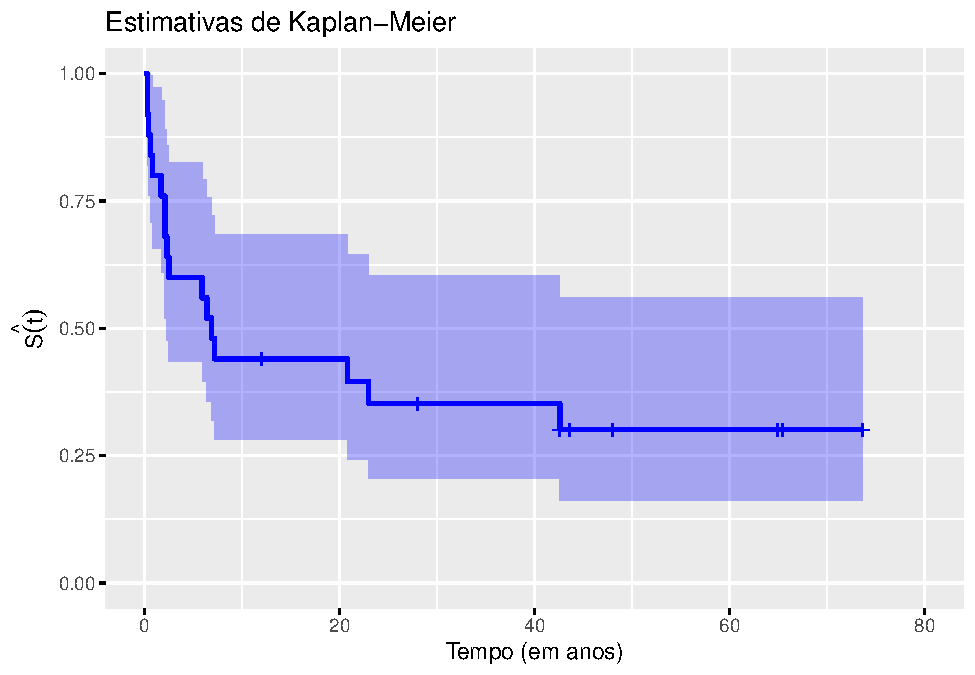
\includegraphics[width=0.8\linewidth]{Lista_3_files/figure-latex/unnamed-chunk-2-1} \end{center}

Por fim é obtido o tamanho amostral, com 5\% e 8\% de nível de
significância do teste e poder igual a 80\%, 85\% e 90\%. Os códigos
estão anexados nesse trabalho.

\begin{longtable}[]{@{}lrr@{}}
\toprule
& 5\% & 8\%\tabularnewline
\midrule
\endhead
80\% & 113.8404 & 97.41371\tabularnewline
85\% & 130.2218 & 112.60848\tabularnewline
90\% & 152.4063 & 133.29933\tabularnewline
\bottomrule
\end{longtable}

\begin{enumerate}
\def\labelenumi{(\alph{enumi})}
\setcounter{enumi}{1}
\tightlist
\item
  Repita o item (a) assumindo que o recrutamento poderá ser feito ao
  longo dos 4 anos e meio. Compare com os resultados do item (a).
\end{enumerate}

\subsection{Resolução}\label{resolucao-1}

O mesmo é feito alterando o tempo de recrutamento para 4 anos e meio:

\begin{longtable}[]{@{}lrr@{}}
\toprule
& 5\% & 8\%\tabularnewline
\midrule
\endhead
80\% & 158.1485 & 135.3284\tabularnewline
85\% & 180.9058 & 156.4371\tabularnewline
90\% & 211.7248 & 185.1811\tabularnewline
\bottomrule
\end{longtable}

Comparando com o item a), o tamanho amostral aumenta se o tempo de
recrutamento aumenta.

\section{Exercício 2}\label{exercicio-2}

Considere \(a_1<...<a_J\) uma partição do eixo do tempo. A função de
sobrevivência da distribuição Exponencial Segmentada (Piecewise
Exponential) é dada por:
\[S(t)=exp\Big \{ -\sum_{j=1}^J \lambda_j \nabla_j(t) \Big \}, \ t>0,\]
em que \[\nabla_j(t)= \left\{ \begin{array}{ll}
0, \ \ \ \ \ \ \ \ \ \ \ \ \ \ \ \ \ \ \ \ se \ t<a_{j-1} \\
t-a_{j-1}, \ \ \ \ \ \ \ \ se \ a_{j-1} \leq t < a_j  \\
a_j - a_{j-1}, \ \ \ \ \ \ se \ t \geq a_j \end{array} \right.\ \] para
\(j=1,...,J\). Defina \(a_0=0\) e \(a_{J+1}=\infty\).

\begin{enumerate}
\def\labelenumi{(\alph{enumi})}
\tightlist
\item
  Mostre que a função de taxa de falha desta distribuição é constante no
  intervalo \((a_j , a_{j+1}), \ \forall \ j=0,1,...,J\).
\end{enumerate}

\subsection{Resolução}\label{resolucao-2}

Sabendo do resultado: \[\alpha(t)=-\frac{d}{dt} ln(S(t))\]

Assim, aplicando o \(ln(.)\) em \(S(t)\), temos:

\[ln(S(t))=ln(exp\Big \{ -\sum_{j=1}^J \lambda_j \nabla_j(t) \Big \})=-\sum_{j=1}^J \lambda_j \nabla_j(t)\]

Dividindo a derivação em 3 casos, temos:

Para o casa em que \(t<a_{j-1} \Rightarrow \nabla_j(t)=0\), logo:

E derivando em relação a \(t\):
\[-\frac{d}{dt} ln(S(t))=-\frac{d}{dt} -\sum_{j=1}^J \lambda_j *0=0\]

Para o casa em que
\(a_{j-1} \leq t < a_j \Rightarrow \nabla_j(t)=t-a_{j-1}\), logo:

E derivando em relação a \(t\):
\[-\frac{d}{dt} ln(S(t))=-\frac{d}{dt} \Big ( -\sum_{j=1}^J \lambda_j (t-a_{j-1}) \Big )= \sum_{j=1}^J \lambda_j\]

Para o casa em que \(t \geq a_j \Rightarrow \nabla_j(t)=a_j - a_{j-1}\),
logo:

E derivando em relação a \(t\):
\[-\frac{d}{dt} ln(S(t))=-\frac{d}{dt} \Big ( -\sum_{j=1}^J \lambda_j (a_j - a_{j-1}) \Big )= 0\]

Com os resultados acima temos que a função de taxa e falha é dada por:
\[\alpha(t)= \left\{ \begin{array}{ll}
0, \ \ \ \ \ \ \ \ \ \ \ \ \ \ \ \ \ \ \ \ se \ t<a_{j-1} \\
\sum_{j=1}^J \lambda_j, \ \ \ \ \ \ \ \ se \ a_{j-1} \leq t < a_j  \\
0, \ \ \ \ \ \ \ \ \ \ \ \ \ \ \ \ \ \ \ \ se \ t \geq a_j \end{array} \right.\ \]

E como a função acima não depende de \(t\), logo é uma função constante.

\begin{enumerate}
\def\labelenumi{(\alph{enumi})}
\setcounter{enumi}{1}
\tightlist
\item
  Para uma amostra (censurada) de tamanho \(n\) desta distribuição,
  mostre que o estimador de máxima verossimilhança do vetor
  \(\boldsymbol{\lambda}=(\lambda_1,...,\lambda_J)\) é dado por
  \(\boldsymbol{\widehat\lambda}=(\widehat\lambda_1,...,\widehat\lambda_J)\),
  com
  \[\widehat\lambda_j=\frac{d_j}{\sum^n_{i=1} \nabla_j(t_i)}, \ j=1,...,J,\]
  em que \(d_j\) representa o número de falhas no j-ésimo intervalo.
\end{enumerate}

\subsection{Resolução}\label{resolucao-3}

\begin{enumerate}
\def\labelenumi{(\alph{enumi})}
\setcounter{enumi}{2}
\tightlist
\item
  Para introduzir covariáveis no modelo, considere a matriz de desenho
  \(\boldsymbol{x}\) sem intercepto. Mostre que esta distribuição
  pertence à classe de modelos de riscos proporcionais em um modelo de
  regressão com \(\lambda_j=exp \{\beta_{0j}+\boldsymbol{x}^T\beta \}\).
\end{enumerate}

\subsection{Resolução}\label{resolucao-4}

Para mostrar que esta distribuição pertence à classe de modelos de
riscos proporcionais em um modelo de regressão, basta mostrar que:
\[\frac{\alpha(t|X_j)}{\alpha(t|X_i)} = k\] Ou seja, a razão acima não
depende de \(t\), para isso, considerando o item a, como apenas para
\(a_{j-1} \leq t < a_j\) em que a função \(\alpha(t)\) é difirente de
zero com \(\alpha(t)=\sum_{j=1}^J \lambda_j\), assim:

\[\frac{\alpha(t|X_j)}{\alpha(t|X_i)} =\frac{\sum_{j=1}^J exp \{\beta_{0j}+\boldsymbol{x}^T\beta \}}{\sum_{i=1}^J exp \{\beta_{0i}+\boldsymbol{x}^T\beta \}}=\frac{\sum_{j=1}^J exp \{\beta_{0j}\} exp\{\boldsymbol{x}^T\beta \}}{\sum_{i=1}^J exp \{\beta_{0i}\} exp\{ \boldsymbol{x}^T\beta \}} =\frac{ exp\{\boldsymbol{x}^T\beta \} \sum_{j=1}^J exp \{\beta_{0j}\}}{ exp\{\boldsymbol{x}^T\beta \}\sum_{i=1}^J exp \{\beta_{0i}\}}=\frac{\sum_{j=1}^J exp \{\beta_{0j}\}}{ \sum_{i=1}^J exp \{\beta_{0i}\}} \ \ \ \ \ (I)\]
Como \((I)\) não depende de \(t\) logo esta distribuição pertence à
classe de modelos de riscos proporcionais em um modelo de regressão com
\(\lambda_j=exp \{\beta_{0j}+\boldsymbol{x}^T\beta \}\).

\section{Exercício 3}\label{exercicio-3}

Os dados no arquivo \textbf{HOD NHL.csv} são referentes a 43 pacientes
com linfoma de Hodgking ou linfoma não Hodgking, submetidos a
transplante de medula óssea. Alguns pacientes receberam transplante de
doador aparentado compatível (transplante alogênico) e outros receberam
transplante autólogo (ou seja, a própria medula óssea do paciente é
coletada e posteriormente infundida). Nos dados também há informação
sobre o escore de Karnofsky, que é uma medida de perfomance que
classifica os pacientes segundo o bem-estar dos pacientes. O objetivo
principal do estudo é a comparação dos tipos de transplante,
considerando-se o tempo (dias) livre de doença (i.e., tempo antes de
ocorrência da recorrência ou óbito).

\begin{enumerate}
\def\labelenumi{(\alph{enumi})}
\tightlist
\item
  Construa curvas de Kaplan-Meier para o tempo de sobrevivência dos
  pacientes com linfoma para cada um dos grupos de tratamento.
  Categorize a variável escore de Karnofsky, criando uma variável com
  duas categorias: escore \textless{} 80 ou escore \(\geq\) 80. Construa
  gráficos de Kaplan-Meier para essa nova variável categorizada.
  Comente.
\end{enumerate}

\subsection{Resolução}\label{resolucao-5}

O estimador Kaplan-Meier para o tempo de sobrevivência dos pacientes com
linfoma para cada um dos grupos de tratamento com intervalo de confiança
de 95\% segue a curva abaixo:

\begin{center}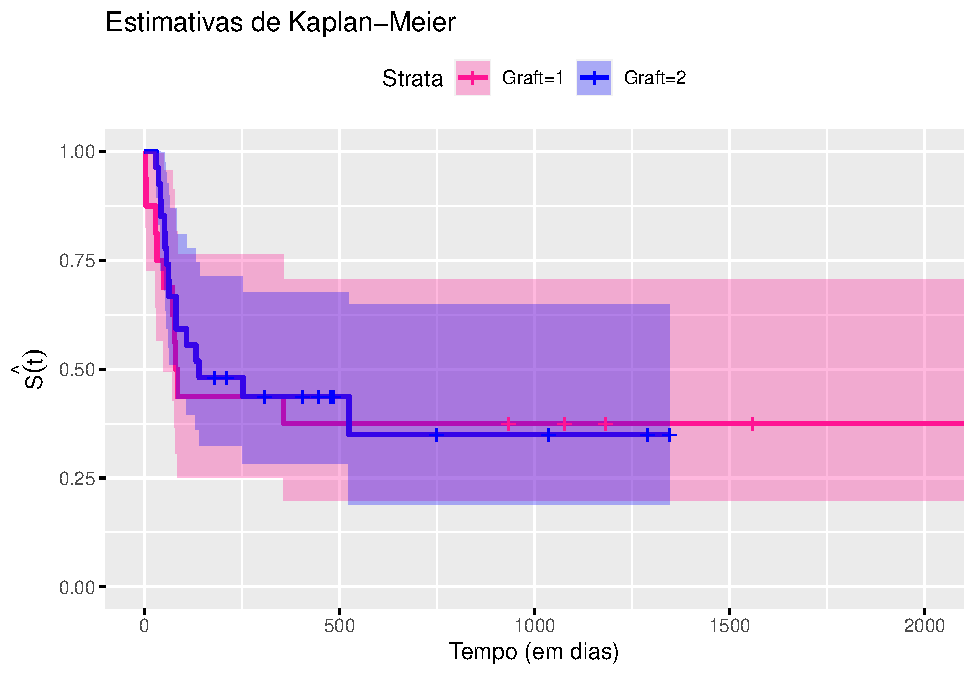
\includegraphics[width=0.8\linewidth]{Lista_3_files/figure-latex/unnamed-chunk-5-1} \end{center}

Em que podemos notar que as curvas de sobrevivência, são bem próximas
para os dois tipos de transplante.

O estimador Kaplan-Meier para o tempo de sobrevivência dos pacientes com
linfoma para cada um dos escore de Karnofsky com intervalo de confiança
de 95\% segue a curva abaixo:

\begin{center}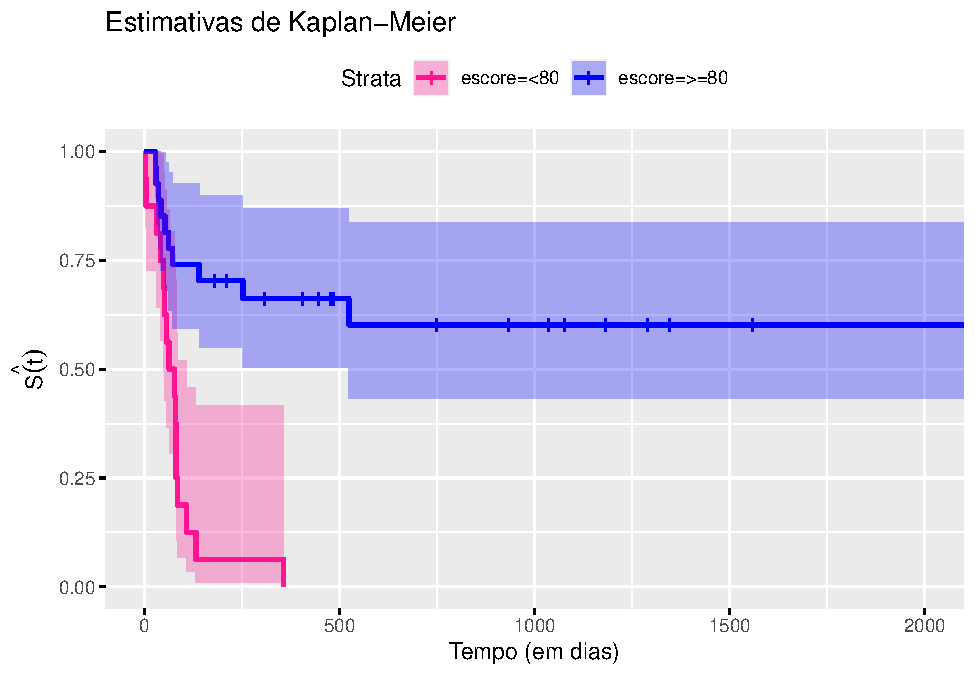
\includegraphics[width=0.8\linewidth]{Lista_3_files/figure-latex/unnamed-chunk-6-1} \end{center}

Em que podemos notar um maior tempo de sobrevivência para os pacientes
com escore de Karnofsky maiores ou iguais a 80, contra os pacientes com
escores menores que 80.

\begin{enumerate}
\def\labelenumi{(\alph{enumi})}
\setcounter{enumi}{1}
\tightlist
\item
  Ajuste um modelo de regressão Weibull com a variável tratamento e a
  variável escore de Karnofsky categorizada conforme o item (a),
  utilizando algum pacote estatístico (R, Splus, SAS, etc.). Apresente
  as estimativas de máxima verossimilhança dos parâmetros considerando a
  representação do modelo Weibull como um modelo de locação-escala e
  também como um modelo de riscos proporcionais.
\end{enumerate}

\subsection{Resolução}\label{resolucao-6}

Utilizando o modelo Weibull com a parametrização locação-escala:
\[Log(T)=\mu +X'\gamma+ \sigma w\] Em que \(\mu\) é o intercepto, \(X\)
é a matriz de covariáveis, \(\gamma\) é o vetor de parâmetros associados
as covariávies (sem intercepto), \(\sigma\) é o parâmetro de escala e
por fim \(w \sim Valor \ Extremo\) padrão. Os parâmetros a serem
estimados são \(\theta=(\mu,\gamma_1,\gamma_2,\sigma)^T\).

Ajustando o modelo obtemos, as estimativas de verossimilhança:

\begin{verbatim}
## 
## Call:
## survreg(formula = Surv(Time, D_R) ~ escore + Graft, data = data, 
##     dist = "weibull")
##              Value Std. Error     z       p
## (Intercept)  5.169      0.908  5.70 1.2e-08
## escore>=80   3.325      0.563  5.91 3.5e-09
## Graft       -0.550      0.525 -1.05    0.29
## Log(scale)   0.263      0.171  1.54    0.12
## 
## Scale= 1.3 
## 
## Weibull distribution
## Loglik(model)= -168.4   Loglik(intercept only)= -183.3
##  Chisq= 29.72 on 2 degrees of freedom, p= 3.5e-07 
## Number of Newton-Raphson Iterations: 5 
## n= 43
\end{verbatim}

E para representação do modelo Weibull como um modelo de riscos
proporcionais, podemos escrever: \[\alpha(t|x)=\alpha_0(t)g(x)\] Sendo
\(g(x)=e^{-x'\gamma/\sigma}\) e \(\alpha_0(t)=\alpha(t|x=0)\) a função
de risco basal, como visto em aula
\[\alpha(t|x)=exp \{ -t^{1/\sigma} e^{-\mu/\sigma} e^{-x'\gamma/\sigma} \} \Rightarrow \alpha_0(t)=\alpha(t|x=0)=exp \{ -t^{1/\sigma} e^{-\mu/\sigma} \}\]
Fazendo \(\beta=-\gamma/\sigma\), e pela invariância do estimador de
máxima verossimilhança temos que as estimativas um modelo weibull de
riscos proporcionais é dado por: \[e^{x'\beta}e^{-\mu/\sigma}\] Assim,
temos:

\begin{longtable}[]{@{}lr@{}}
\toprule
Variaveis & estimativa\tabularnewline
\midrule
\endhead
Intercepto & 0.0188111\tabularnewline
escore\textgreater{}=80 & 0.0776272\tabularnewline
Graft & 1.5262664\tabularnewline
\bottomrule
\end{longtable}

\begin{enumerate}
\def\labelenumi{(\alph{enumi})}
\setcounter{enumi}{2}
\tightlist
\item
  Encontre uma estimativa pontual para a razão de taxas de falha de
  pacientes que receberam transplante autólogo e alogênico. Encontre
  também uma estimativa do fator de aceleração, deixando claro como foi
  calculado. Faça o mesmo para a outra variável (escore de Karnofsky)
  incluída no modelo.
\end{enumerate}

\subsection{Resolução}\label{resolucao-7}

Para os pacientes que receberam transplante autólogo \(Graft=2\) e
alogênico \(Graft=1\), temos:
\[\frac{\alpha(t|Graft=1)}{\alpha(t|Graft=2)}=\frac{e^{5.17}}{e^{5.17-0.55}}=\frac{175.91}{101.494}=1.73\]
Ou seja, risco de indivíduo que recebeu o transplante alogênico morrer é
1.73 vezes maior do que o de morrer com o transplante autólogo.

O modelo de vida acelerado é dado por: \[S(t|x)=S_0(\psi_xt)\]

Como visto em aula, o fator de aceleração é dado por:
\[\psi_x=e^{-x'\gamma}=e^{-\gamma_1x_1}=e^{0.55*1}=1.1733\]

Ou seja, como \(\phi_x>1\), temos que para os pacientes que receberam
transplante autólogo se comportam como `passado' do que os pacientes que
receberam transplante alogênico.

Para os pacientes que com escores Karnofsky \textgreater{}=80 e com
escores \textless{}80, temos:
\[\frac{\alpha(t|"escore<80"=1)}{\alpha(t|"escore<80"=0)}=\frac{e^{5.17+3.325}}{e^{5.17}}=\frac{4890.25}{175.91}=27.8\]
Ou seja, risco de indivíduo que tem o escore de Karnofsky \textless{}80
morrer é 27.8 vezes maior do que quem tem o escore de Karnofsky
\textgreater{}=80.

Como visto em aula, o fator de aceleração é dado por:
\[\psi_x=e^{-x'\gamma}=e^{-\gamma_1x_1}=e^{-3.325*1}=0.036\]

Ou seja, como \(\phi_x<1\), temos que para os pacientes que tem escore
de Karnofsky \textless{}80 se comportam como `futuro' do que os
pacientes que tem escore de Karnofsky \textgreater{}=80.

\begin{enumerate}
\def\labelenumi{(\alph{enumi})}
\setcounter{enumi}{3}
\tightlist
\item
  Teste a hipótese de igualdade dos tipos de transplante e também das
  categorias do escore de Karnofsky, utilizando a estatística de Wald,
  com um nível de significância de 10\%. Comente.
\end{enumerate}

\subsection{Resolução}\label{resolucao-8}

Para testar a igualdade dos transplante é equivalente a testar se os
parâmetros da regressão são iguais a zero, ou seja:
\[ \left\{ \begin{array}{ll}
H_0: \gamma_i=0 \ com \ i=1,2 \\
H_1: \gamma_i \ne 0  \end{array} \right.\ \]

E para isso a estatística de Wald é dada por:
\[\frac{\hat\gamma-\gamma}{\sqrt{I^{-1}(\gamma)}}\] em que
\(I^{-1}(\gamma)\) é a variância de \(\gamma\) obtida através da matriz
de informação de fisher. Assim, sob \(H_0\), temos:

\begin{longtable}[]{@{}lrrrr@{}}
\toprule
& Value & Std. Error & z & p\tabularnewline
\midrule
\endhead
(Intercept) & 5.1692031 & 0.9076140 & 5.695376 &
0.0000000\tabularnewline
escore\textgreater{}=80 & 3.3250980 & 0.5630723 & 5.905277 &
0.0000000\tabularnewline
Graft & -0.5500871 & 0.5247505 & -1.048283 & 0.2945082\tabularnewline
Log(scale) & 0.2631195 & 0.1706529 & 1.541840 & 0.1231125\tabularnewline
\bottomrule
\end{longtable}

Em que podemos notar que para variável escore de Karnofsky as categorias
são diferentes com um nível de significâcia de 5\%, porém para a
variável Graft, isso não o ocorre, logo com um nível de significâcia de
5\%, os tipos de transplantes são iguais.

\section{Exercício 4}\label{exercicio-4}

Considere os dados do exercício 3.

\begin{enumerate}
\def\labelenumi{(\alph{enumi})}
\tightlist
\item
  Refaça o item (b) utilizando a distribuição log-logística. Especifique
  claramente qual foi o modelo utilizado e quais foram os parâmetros
  estimados.
\end{enumerate}

\subsection{Resolução}\label{resolucao-9}

Utilizando o modelo log-losgistico com a parametrização locação-escala:
\[Log(T)=\mu +X'\gamma+ \sigma w\]

Em que \(\mu\) é o intercepto, \(X\) é a matriz de covariáveis,
\(\gamma\) é o vetor de parâmetros associados as covariávies (sem
intercepto), \(\sigma\) é o parâmetro de escala e por fim
\(w \sim Logistica\) padrão.Os parâmetros a serem estimados são
\(\theta=(\mu,\gamma_1,\gamma_2,\sigma)^T\).

Ajustando o modelo obtemos:

\begin{verbatim}
## 
## Call:
## survreg(formula = Surv(Time, D_R) ~ escore + Graft, data = data, 
##     dist = "loglogistic")
##               Value Std. Error     z       p
## (Intercept)  4.5807     1.1040  4.15 3.3e-05
## escore>=80   2.8753     0.6480  4.44 9.1e-06
## Graft       -0.3547     0.6519 -0.54    0.59
## Log(scale)   0.0922     0.1688  0.55    0.58
## 
## Scale= 1.1 
## 
## Log logistic distribution
## Loglik(model)= -170.9   Loglik(intercept only)= -180.2
##  Chisq= 18.56 on 2 degrees of freedom, p= 9.3e-05 
## Number of Newton-Raphson Iterations: 4 
## n= 43
\end{verbatim}

\begin{enumerate}
\def\labelenumi{(\alph{enumi})}
\setcounter{enumi}{1}
\tightlist
\item
  Encontre uma estimativa pontual para ao fator de aceleração e
  interprete o resultado.
\end{enumerate}

\subsection{Resolução}\label{resolucao-10}

O modelo de vida acelerado é dado por: \[S(t|x)=S_0(\psi_xt)\]

Como visto em aula, o fator de aceleração é dado por:
\[\psi_x=e^{-x'\gamma}=e^{-\gamma_1x_1-\gamma_2x_2}=e^{-3.325x_1+0.55x_2}\]

\begin{enumerate}
\def\labelenumi{(\alph{enumi})}
\setcounter{enumi}{2}
\tightlist
\item
  A chance de sobrevivência após \(t\) é definida como
  \[\frac{S(t|x)}{1-S(t|x)}\] No modelo logístico, mostre que:
  \[\frac{S(t|x)}{1-S(t|x)}=exp[-x^T \beta]\frac{S(t|x=0)}{1-S(t|x=0)}\]
\end{enumerate}

\subsection{Resolução}\label{resolucao-11}

Sabemos que o modelo log-logístico é definido como:
\[Log(T)=\mu +x'\gamma+ \sigma w\] com \(w\sim Logistica\) padrão.
Assim:

\[\frac{S(t|x)}{1-S(t|x)}=\frac{\mathbb{P}(T>t|x)}{1-\mathbb{P}(T>t|x)}=\frac{\mathbb{P}(T>t|x)}{\mathbb{P}(T \le t|x)}=\frac{\mathbb{P}(ln(T)>ln(t|x))}{\mathbb{P}(ln(T) \le ln(t|x))}=\frac{\mathbb{P}(\mu+x'\gamma+ \sigma w>ln(t|x))}{\mathbb{P}(\mu+x'\gamma+ \sigma w \le ln(t|x))}\]

\[\Rightarrow \frac{S(t|x)}{1-S(t|x)}=\frac{\mathbb{P}( w>(ln(t)-\mu-x'\gamma)/\sigma)}{\mathbb{P}( w \le (ln(t)-\mu-x'\gamma)/\sigma)}=\frac{\frac{1}{1+ e^{(ln(t)-\mu-x'\gamma)/\sigma}}}{\frac{e^{(ln(t)-\mu-x'\gamma)/\sigma}}{1+ e^{(ln(t)-\mu-x'\gamma)/\sigma}}}=\frac{1}{e^{(ln(t)-\mu-x'\gamma)/\sigma}}=t^{1/\sigma}e^{-\mu-x'\gamma/\sigma}\]
Definindo \(e^{x'\gamma/\sigma}\) como \(e^{x'\beta}\)

\[\Rightarrow \frac{S(t|x)}{1-S(t|x)}=t^{1/\sigma}e^{-\mu/\sigma}e^{-x'\beta} \ \ \ \ (I)\]
Pelo resultado de \((I)\) temos que:
\[\frac{S(t|x=0)}{1-S(t|x=0)}=t^{1/\sigma}e^{-\mu/\sigma}\] Logo:
\[\frac{S(t|x)}{1-S(t|x)}=exp[-x^T \beta]\frac{S(t|x=0)}{1-S(t|x=0)}\]

\begin{enumerate}
\def\labelenumi{(\alph{enumi})}
\setcounter{enumi}{3}
\tightlist
\item
  Obtenha uma estimativa da razão de chances de sobrevivência após \(t\)
  de pacientes com células anormais e pacientes com células normais.
  Interprete.
\end{enumerate}

\subsection{Resolução}\label{resolucao-12}

\begin{enumerate}
\def\labelenumi{(\alph{enumi})}
\setcounter{enumi}{4}
\tightlist
\item
  Repita o item (d) do exercício 3, utilizando o modelo log-logístico.
  Compare os resultados e comente.
\end{enumerate}

\subsection{Resolução}\label{resolucao-13}

\section{Exercício 5}\label{exercicio-5}

Considerando ainda os dados do exercício 3, faça gráficos apropriados da
taxa de falha acumulada para verificar a adequabilidade dos modelos.

Em todos os casos, utilize o estimador de Nelson-Aalen da função de taxa
de falha acumulada considerando cada grupo separadamente (ou seja,
obtenha estimativas da função de taxa de falha acumulada para cada
grupo).

\begin{enumerate}
\def\labelenumi{(\alph{enumi})}
\tightlist
\item
  Weibull
\end{enumerate}

\subsection{Resolução}\label{resolucao-14}

\begin{center}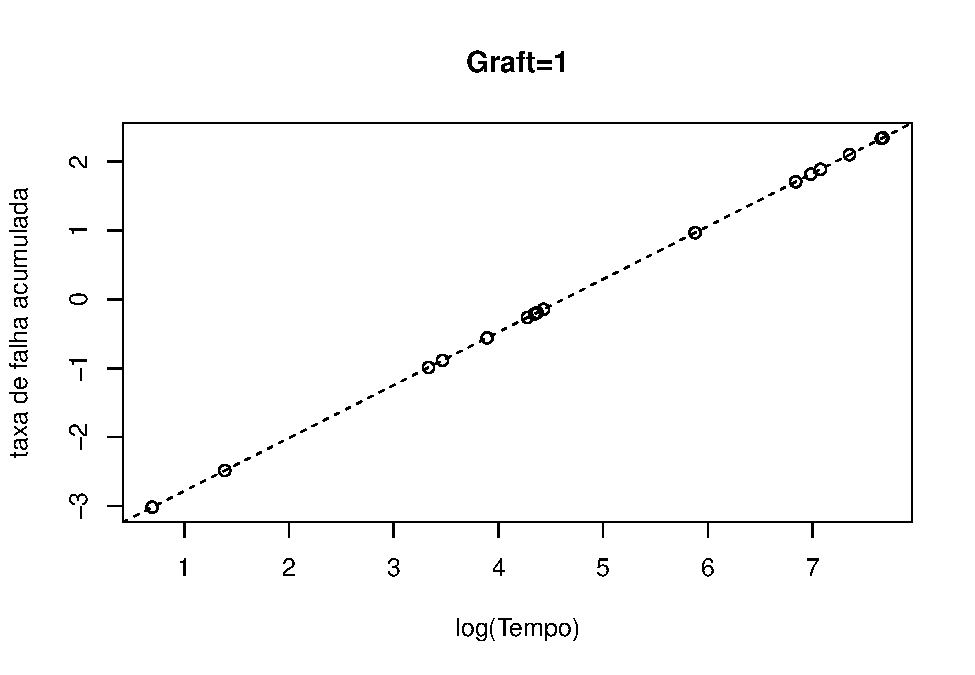
\includegraphics[width=0.8\linewidth]{Lista_3_files/figure-latex/unnamed-chunk-13-1} \end{center}

\begin{center}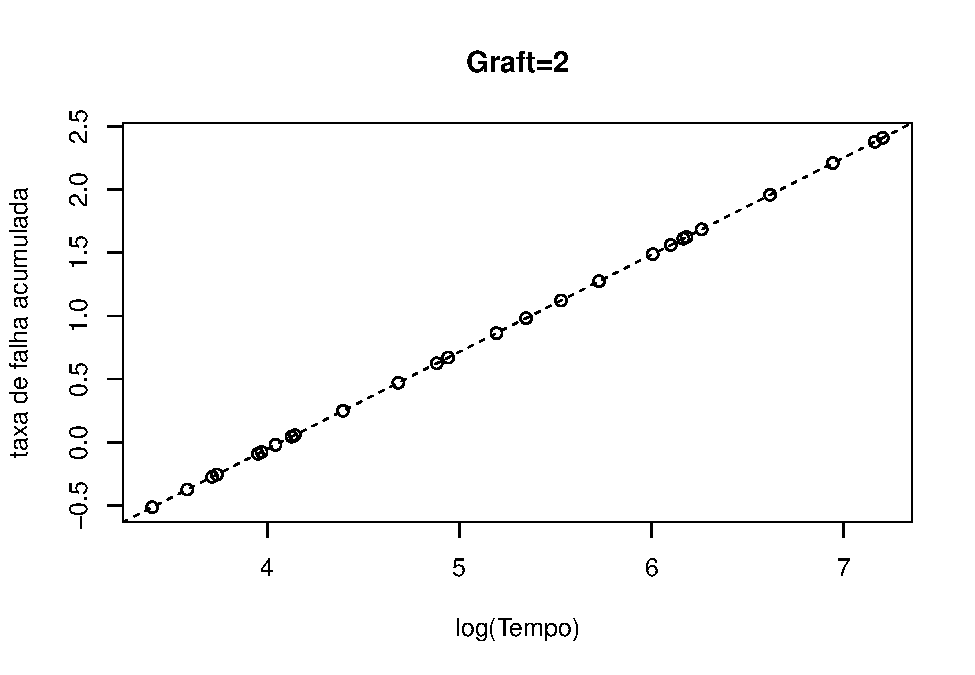
\includegraphics[width=0.8\linewidth]{Lista_3_files/figure-latex/unnamed-chunk-13-2} \end{center}

Pode-se observar que os pontos passam por uma reta com uma certa
inclinação que cruza a origem.

\begin{enumerate}
\def\labelenumi{(\alph{enumi})}
\setcounter{enumi}{1}
\tightlist
\item
  Log-logístico
\end{enumerate}

\subsection{Resolução}\label{resolucao-15}

\begin{center}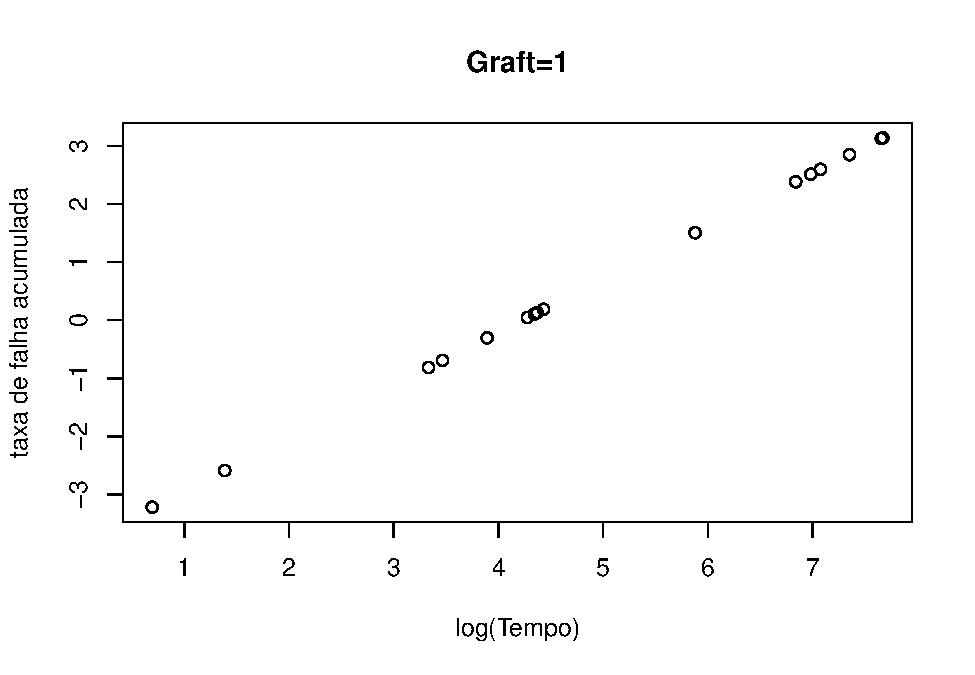
\includegraphics[width=0.8\linewidth]{Lista_3_files/figure-latex/unnamed-chunk-14-1} \end{center}

\begin{center}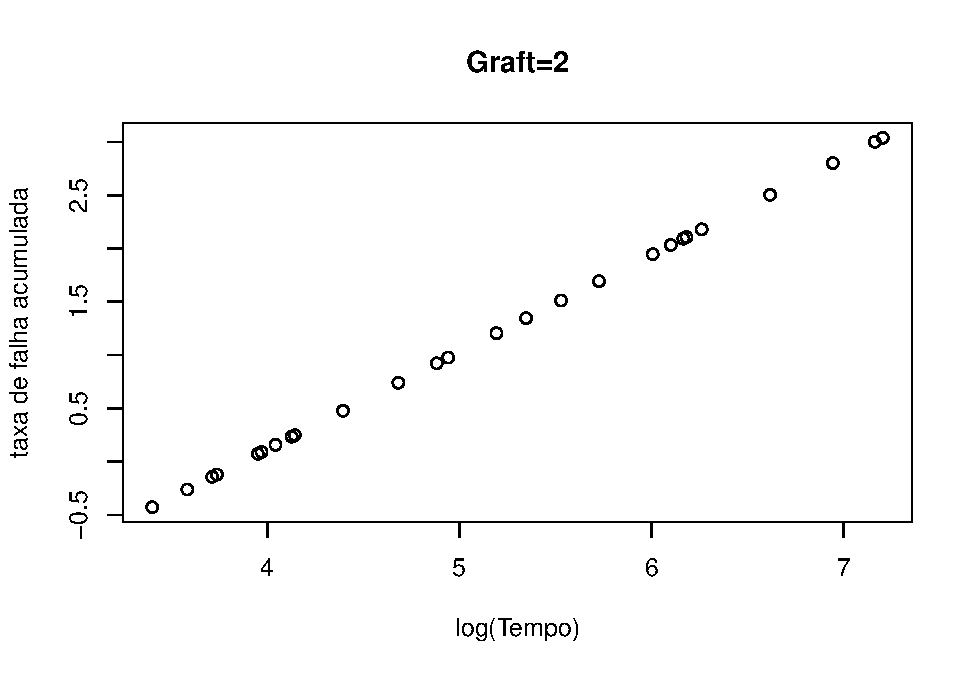
\includegraphics[width=0.8\linewidth]{Lista_3_files/figure-latex/unnamed-chunk-14-2} \end{center}

Era de se esperar que os pontos formassem uma reta. Logo os dois modelos
aparentam adequados.

\section{Exercício 6}\label{exercicio-6}

Considere ainda os dados do exercício 3. Obtenha os resíduos de
Cox-Snell e \emph{deviance} para os modelos de regressão Weibull
(ajustado no exercício 4) e log-logístico (ajustado no exercício 3).
Faça gráficos dos resíduos em função do tempo e comente. Com base em
todas as análises feitas, discuta se os modelos (Weibull ou
log-logístico) parecem ser adequados para os dados trabalhados.

A partir dos dados do arquivo \textbf{HOD NHL.csv}, os resíduos de
Cox-Snell para o modelo Weibull são obtidos a seguir:

\begin{verbatim}
##  [1]  0.56758764  0.41207674  0.57176005  0.86525054  2.63119525
##  [6]  8.40377759  9.39068861 10.08613452 12.47585343 15.75857694
## [11] 15.93019088  0.04891378  0.08333317  1.17304200  0.80927421
## [16]  0.82538328  0.06017272  0.07195380  0.04985537  0.05384209
## [21]  0.06531543  0.15181352  0.06531543  0.23852048  0.41870020
## [26]  0.20733041  0.38889446  0.70756696  0.04645991  0.05344918
## [31]  0.03870126  0.04645845  0.08117288  0.08147980  0.09506879
## [36]  0.18416384  0.27760551  0.34413806  0.36991370  0.39390869
## [41]  0.55044465  0.83684300  0.86413500
\end{verbatim}

Os resíduos de Cox-Snell para o modelo log-logístico também são obtidos:

\begin{verbatim}
##  [1] 0.47725849 0.40542613 0.55234918 0.79089565 1.70650452 2.77037407
##  [7] 2.89434298 2.97459303 3.21540094 3.48275921 3.49521670 0.03911720
## [13] 0.07237462 0.89495811 0.74831050 0.76069769 0.06233804 0.07651805
## [19] 0.05967755 0.06519823 0.08132414 0.17632690 0.08132414 0.28485768
## [25] 0.49621705 0.24614999 0.46285485 0.78722442 0.04624097 0.05438128
## [31] 0.04452922 0.05501419 0.08778073 0.10448254 0.12420825 0.21711935
## [37] 0.33259335 0.41153265 0.44126861 0.46851314 0.63596133 0.90057648
## [43] 0.92335361
\end{verbatim}

Os resíduos \emph{deviance} também são obtidos para o modelo Weibull:

\begin{verbatim}
##  [1]  0.5175862  0.7728162  0.5114605  0.1413274 -1.1521780 -4.0997018
##  [7] -4.3337486 -4.4913549 -4.9951684 -5.6140141 -5.6445001  2.0330322
## [13]  1.7710120 -0.1639611  0.2044098  0.1859607  1.9342745  1.8459062
## [19]  2.0240970  1.9877333  1.8941185  1.4400805  1.8941185  1.1591554
## [25]  0.7606580 -0.6439416 -0.8819234 -1.1895940  2.0570005  1.9912173
## [31]  2.1403665  2.0570150  1.7845710  1.7826272  1.7018950 -0.6069001
## [37] -0.7451248 -0.8296241 -0.8601322 -0.8875908 -1.0492327 -1.2937102
## [43] -1.3146368
\end{verbatim}

e para o modelo log-logístico:

\begin{verbatim}
##  [1]  0.6587192  0.7851659  0.5402297  0.2257649 -0.5866130 -2.3538794
##  [7] -2.4059688 -2.4390953 -2.5359026 -2.6392269 -2.6439428  2.1355609
## [13]  1.8429727  0.1089631  0.2765783  0.2615987  1.9170401  1.8147984
## [19]  1.9382864  1.8950046  1.7836123  1.3503648  1.7836123  1.0398300
## [25]  0.6276287 -0.7016409 -0.9621381 -1.2547704  2.0591891  1.9829859
## [31]  2.0766024  1.9774622  1.7439576  1.6511922  1.5556375 -0.6589679
## [37] -0.8155898 -0.9072295 -0.9394345 -0.9680012 -1.1277955 -1.3420704
## [43] -1.3589361
\end{verbatim}

Com esses resultados, é possível elaborar gráficos desses resíduos para
a análise da escolha do modelo. Uma opção é realizar um gráfico da
função de risco acumulada para os resíduos de Cox-Snell, utilizando os
estimadores de Kaplan-Meier (em vermelho) e Nelson\_Aalen (em azul),
primeiramente para o modelo Weibull:

\begin{center}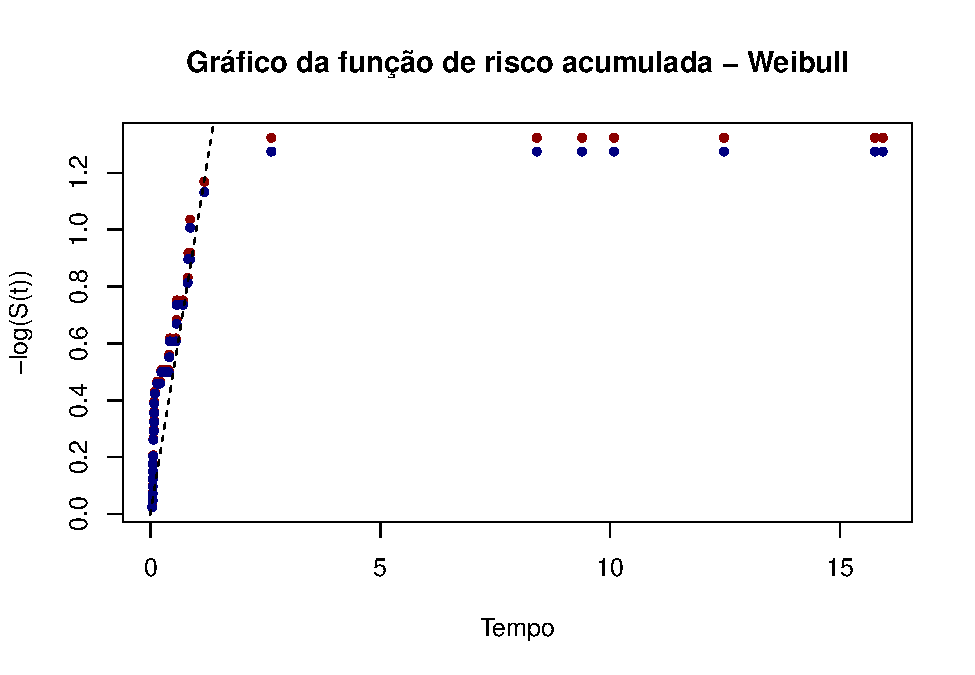
\includegraphics[width=0.8\linewidth]{Lista_3_files/figure-latex/unnamed-chunk-19-1} \end{center}

O mesmo é feito para o modelo log-logístico:

\begin{center}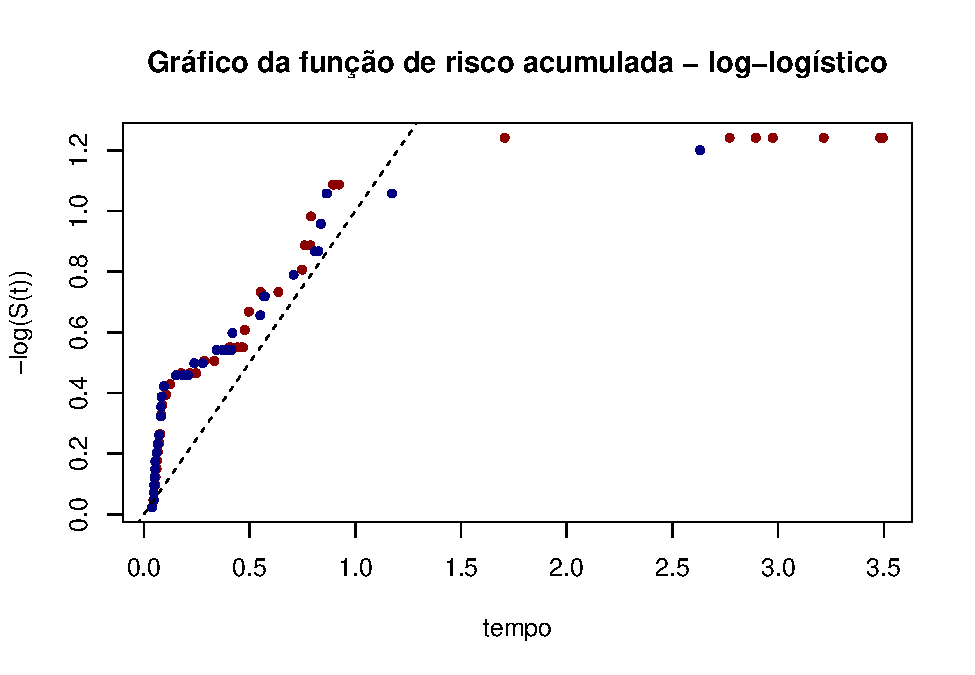
\includegraphics[width=0.8\linewidth]{Lista_3_files/figure-latex/unnamed-chunk-20-1} \end{center}

O esperado é que os resíduos acompanhem a linha pontilhada. Graficando
os resíduos deviance em relação ao tempo para o modelo Weibull:

\begin{center}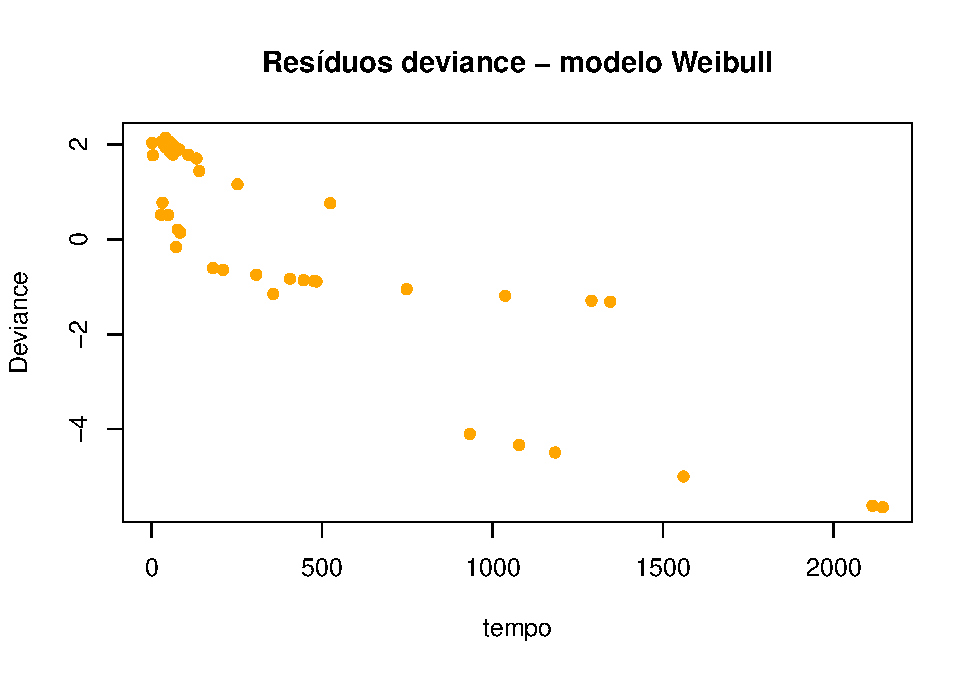
\includegraphics[width=0.8\linewidth]{Lista_3_files/figure-latex/unnamed-chunk-21-1} \end{center}

O mesmo processo para o modelo log-logístico:

\begin{center}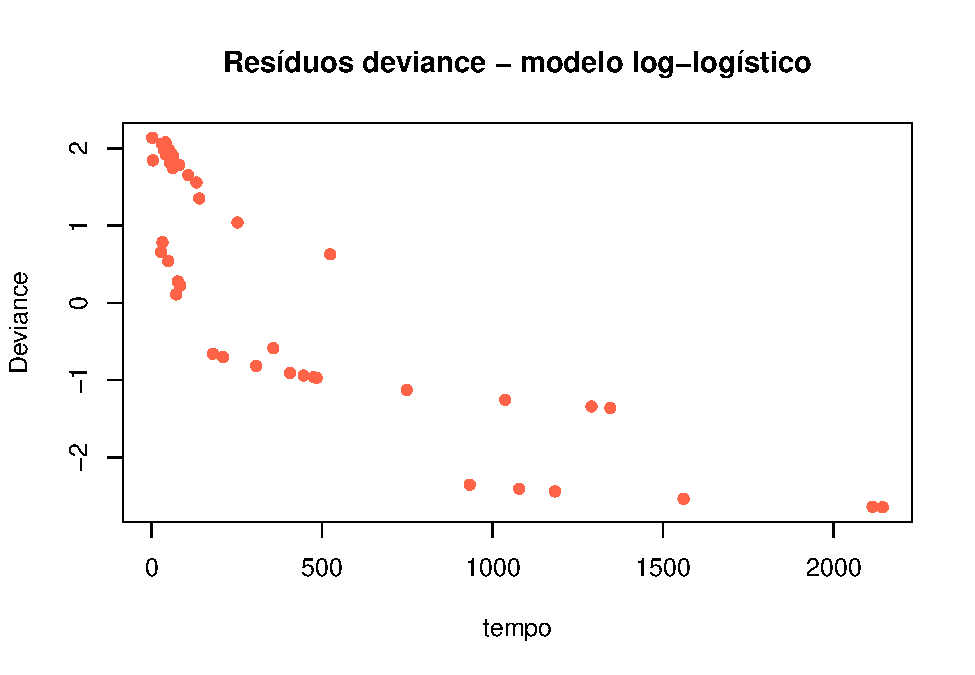
\includegraphics[width=0.8\linewidth]{Lista_3_files/figure-latex/unnamed-chunk-22-1} \end{center}

Para interpretar esses gráficos é necessário verificar se os pontos
estão próximos ou mais distantes entre si, quanto mais próximos melhor o
ajuste do modelo. Logo, nota-se que pelos gráficos do resíduos de
Cox-Snell, o modelo Weibull possuem os primeiros pontos mais próximos da
reta pontilhada do que o modelo log-logístico. Pelos gráficos dos
resíduos deviance pode-se dizer que os resíduos estão mais concentrados
para o modelo log-logístico, dos quais variam de -3 e 3, do que os
resíduos para o modelo Weibull variam de -6 e 3, entretanto os dois
possuem pontos bem distântes entre si. Portanto, pode-se dizer que o
modelo Weibull aparentemente está melhor ajustado. Pode-se fazer os
cretérios AIC e BIC para confirmar a escolha. O AIC para o modelo
Weibull é de 344.8589 e para o modelo log-logístico é 349.8397. O BIC
para o modelo Weibull é de -174,0712 e para o modelo log-logístico é
-176.5617. Observando o menor AIC e o maior BIC, confirma-se que o
modelo Weibull está melhor ajustado.

\section{Anexo}\label{anexo}

\subsection{Códigos}\label{codigos}

\begin{Shaded}
\begin{Highlighting}[]
 \CommentTok{# Pacotes}
\KeywordTok{library}\NormalTok{(ggplot2)}
\KeywordTok{library}\NormalTok{(asaur)}
\KeywordTok{library}\NormalTok{(survival)}
\KeywordTok{library}\NormalTok{(survminer)}
\KeywordTok{library}\NormalTok{(sqldf)}
\KeywordTok{library}\NormalTok{(mice)}
\KeywordTok{library}\NormalTok{(KMsurv)}
\KeywordTok{library}\NormalTok{(mice)}


\CommentTok{# Exercício 1}

\CommentTok{# item a}
\NormalTok{Tempo <-}\StringTok{ }\KeywordTok{c}\NormalTok{(}\FloatTok{0.3}\NormalTok{,}\FloatTok{5.9}\NormalTok{,}\FloatTok{20.8}\NormalTok{,}\FloatTok{28.0}\NormalTok{,}\FloatTok{1.7}\NormalTok{,}\FloatTok{73.6}\NormalTok{,}\FloatTok{7.2}\NormalTok{,}\FloatTok{2.1}\NormalTok{,}\FloatTok{6.4}\NormalTok{,}\FloatTok{2.5}\NormalTok{,}\FloatTok{2.3}\NormalTok{,}\FloatTok{0.3}\NormalTok{,}\FloatTok{0.4}\NormalTok{,}\FloatTok{65.4}\NormalTok{,}\FloatTok{64.9}\NormalTok{,}\FloatTok{0.6}\NormalTok{,}\FloatTok{23.0}\NormalTok{,}\FloatTok{42.6}\NormalTok{,}\FloatTok{48.0}\NormalTok{,}\FloatTok{6.9}\NormalTok{,}\FloatTok{2.1}\NormalTok{,}\FloatTok{43.6}\NormalTok{,}\FloatTok{42.6}\NormalTok{,}\FloatTok{12.0}\NormalTok{,}\FloatTok{0.8}\NormalTok{)}
\NormalTok{Censura <-}\StringTok{ }\KeywordTok{c}\NormalTok{(}\DecValTok{1}\NormalTok{,}\DecValTok{1}\NormalTok{,}\DecValTok{1}\NormalTok{,}\DecValTok{0}\NormalTok{,}\DecValTok{1}\NormalTok{,}\DecValTok{0}\NormalTok{,}\DecValTok{1}\NormalTok{,}\DecValTok{1}\NormalTok{,}\DecValTok{1}\NormalTok{,}\DecValTok{1}\NormalTok{,}\DecValTok{1}\NormalTok{,}\DecValTok{1}\NormalTok{,}\DecValTok{1}\NormalTok{,}\DecValTok{0}\NormalTok{,}\DecValTok{0}\NormalTok{,}\DecValTok{1}\NormalTok{,}\DecValTok{1}\NormalTok{,}\DecValTok{0}\NormalTok{,}\DecValTok{0}\NormalTok{,}\DecValTok{1}\NormalTok{,}\DecValTok{1}\NormalTok{,}\DecValTok{0}\NormalTok{,}\DecValTok{1}\NormalTok{,}\DecValTok{0}\NormalTok{,}\DecValTok{1}\NormalTok{)}

\KeywordTok{library}\NormalTok{(survival)}
\KeywordTok{library}\NormalTok{(survminer)}
\NormalTok{Ex1 <-}\StringTok{ }\KeywordTok{data.frame}\NormalTok{(Tempo,Censura)}

\NormalTok{KM1 <-}\StringTok{ }\KeywordTok{survfit}\NormalTok{(}\KeywordTok{Surv}\NormalTok{(Ex1}\OperatorTok{$}\NormalTok{Tempo, Ex1}\OperatorTok{$}\NormalTok{Censura)}\OperatorTok{~}\DecValTok{1}\NormalTok{)}


\CommentTok{# Tabela com estimativas de Kaplan-Meier}
\NormalTok{knitr}\OperatorTok{::}\KeywordTok{kable}\NormalTok{(}\KeywordTok{surv_summary}\NormalTok{(KM1),}\DataTypeTok{col.names =} \KeywordTok{c}\NormalTok{(}\StringTok{"Tempo"}\NormalTok{,}\StringTok{"nº em risco"}\NormalTok{,}\StringTok{"nº de eventos"}\NormalTok{,}
                                             \StringTok{"censura"}\NormalTok{,}\StringTok{"sobreviv."}\NormalTok{,}\StringTok{"desv.pad sobrev."}\NormalTok{,}
                                             \StringTok{"IC(95%) sup."}\NormalTok{,}\StringTok{"IC(95%) inf."}\NormalTok{))}

\CommentTok{# Grafico Kaplan-Meier}
\KeywordTok{ggsurvplot}\NormalTok{(KM1, }\DataTypeTok{data =}\NormalTok{ Ex1,}\DataTypeTok{palette =} \KeywordTok{c}\NormalTok{(}\StringTok{'blue'}\NormalTok{),}
           \DataTypeTok{ggtheme=}\KeywordTok{theme_gray}\NormalTok{(), }\DataTypeTok{legend =} \StringTok{'none'}\NormalTok{) }\OperatorTok{+}\StringTok{ }
\StringTok{  }\KeywordTok{labs}\NormalTok{(}\DataTypeTok{x=}\StringTok{"Tempo (em anos)"}\NormalTok{,}
       \DataTypeTok{y=}\KeywordTok{expression}\NormalTok{(}\KeywordTok{hat}\NormalTok{(}\KeywordTok{S}\NormalTok{(t))),}
       \DataTypeTok{title =} \StringTok{"Estimativas de Kaplan-Meier"}\NormalTok{) }

\NormalTok{x <-}\StringTok{ }\NormalTok{(}\DecValTok{18}\OperatorTok{-}\DecValTok{12}\NormalTok{)}\OperatorTok{/}\NormalTok{((}\FloatTok{20.8}\OperatorTok{-}\DecValTok{12}\NormalTok{)}\OperatorTok{/}\NormalTok{(}\FloatTok{0.396}\OperatorTok{-}\FloatTok{0.44}\NormalTok{))}\OperatorTok{+}\FloatTok{0.44}

\CommentTok{#log(0.65)/log(0.41)}

\CommentTok{#log(0.4831582)}

\CommentTok{# a =5% b= 80%}
\NormalTok{d <-}\StringTok{ }\KeywordTok{data.frame}\NormalTok{()}
\NormalTok{d[}\DecValTok{1}\NormalTok{,}\DecValTok{1}\NormalTok{] =}\StringTok{ }\DecValTok{4}\OperatorTok{*}\NormalTok{(}\FloatTok{1.96}\OperatorTok{+}\FloatTok{0.8416}\NormalTok{)}\OperatorTok{^}\DecValTok{2}\OperatorTok{/}\NormalTok{(}\OperatorTok{-}\FloatTok{0.7274111}\NormalTok{)}\OperatorTok{^}\DecValTok{2}

\CommentTok{# a = 8% b = 80%}
\NormalTok{d[}\DecValTok{1}\NormalTok{,}\DecValTok{2}\NormalTok{] =}\StringTok{ }\DecValTok{4}\OperatorTok{*}\NormalTok{(}\FloatTok{1.75}\OperatorTok{+}\FloatTok{0.8416}\NormalTok{)}\OperatorTok{^}\DecValTok{2}\OperatorTok{/}\NormalTok{(}\OperatorTok{-}\FloatTok{0.7274111}\NormalTok{)}\OperatorTok{^}\DecValTok{2}

\CommentTok{# a =5% b= 85%}
\NormalTok{d[}\DecValTok{2}\NormalTok{,}\DecValTok{1}\NormalTok{] =}\StringTok{ }\DecValTok{4}\OperatorTok{*}\NormalTok{(}\FloatTok{1.96}\OperatorTok{+}\FloatTok{1.0364}\NormalTok{)}\OperatorTok{^}\DecValTok{2}\OperatorTok{/}\NormalTok{(}\OperatorTok{-}\FloatTok{0.7274111}\NormalTok{)}\OperatorTok{^}\DecValTok{2}

\CommentTok{# a = 8% b = 85%}
\NormalTok{d[}\DecValTok{2}\NormalTok{,}\DecValTok{2}\NormalTok{] =}\StringTok{ }\DecValTok{4}\OperatorTok{*}\NormalTok{(}\FloatTok{1.75}\OperatorTok{+}\FloatTok{1.0364}\NormalTok{)}\OperatorTok{^}\DecValTok{2}\OperatorTok{/}\NormalTok{(}\OperatorTok{-}\FloatTok{0.7274111}\NormalTok{)}\OperatorTok{^}\DecValTok{2}

\CommentTok{# a =5% b= 90%}
\NormalTok{d[}\DecValTok{3}\NormalTok{,}\DecValTok{1}\NormalTok{] =}\StringTok{ }\DecValTok{4}\OperatorTok{*}\NormalTok{(}\FloatTok{1.96}\OperatorTok{+}\FloatTok{1.2816}\NormalTok{)}\OperatorTok{^}\DecValTok{2}\OperatorTok{/}\NormalTok{(}\OperatorTok{-}\FloatTok{0.7274111}\NormalTok{)}\OperatorTok{^}\DecValTok{2}

\CommentTok{# a = 8% b = 90%}
\NormalTok{d[}\DecValTok{3}\NormalTok{,}\DecValTok{2}\NormalTok{] =}\StringTok{ }\DecValTok{4}\OperatorTok{*}\NormalTok{(}\FloatTok{1.75}\OperatorTok{+}\FloatTok{1.2816}\NormalTok{)}\OperatorTok{^}\DecValTok{2}\OperatorTok{/}\NormalTok{(}\OperatorTok{-}\FloatTok{0.7274111}\NormalTok{)}\OperatorTok{^}\DecValTok{2}

\NormalTok{a=}\StringTok{ }\DecValTok{2}

\NormalTok{S30 <-}\StringTok{ }\NormalTok{(}\DecValTok{30}\OperatorTok{-}\DecValTok{28}\NormalTok{)}\OperatorTok{/}\NormalTok{((}\FloatTok{42.6}\OperatorTok{-}\DecValTok{28}\NormalTok{)}\OperatorTok{/}\NormalTok{(}\FloatTok{0.3017143}\OperatorTok{-}\FloatTok{0.3520000}\NormalTok{))}\OperatorTok{+}\FloatTok{0.3520000}
\NormalTok{S42 <-}\StringTok{ }\NormalTok{(}\DecValTok{42}\OperatorTok{-}\DecValTok{28}\NormalTok{)}\OperatorTok{/}\NormalTok{((}\FloatTok{42.6}\OperatorTok{-}\DecValTok{28}\NormalTok{)}\OperatorTok{/}\NormalTok{(}\FloatTok{0.3017143}\OperatorTok{-}\FloatTok{0.3520000}\NormalTok{))}\OperatorTok{+}\FloatTok{0.3520000}
\NormalTok{S54 <-}\StringTok{ }\FloatTok{0.3017143}
\NormalTok{ppad <-}\StringTok{ }\DecValTok{1}\OperatorTok{-}\NormalTok{(S30}\OperatorTok{+}\DecValTok{4}\OperatorTok{*}\NormalTok{S42}\OperatorTok{+}\StringTok{ }\NormalTok{S54)}\OperatorTok{/}\DecValTok{6}

\NormalTok{S30N <-}\StringTok{ }\NormalTok{S30}\OperatorTok{^-}\KeywordTok{log}\NormalTok{(ppad)}
\NormalTok{S42N <-}\StringTok{ }\NormalTok{S42}\OperatorTok{^-}\KeywordTok{log}\NormalTok{(ppad)}
\NormalTok{S54N <-}\StringTok{ }\NormalTok{S54}\OperatorTok{^-}\KeywordTok{log}\NormalTok{(ppad)}

\NormalTok{pnovo <-}\StringTok{ }\DecValTok{1}\OperatorTok{-}\NormalTok{(S30N}\OperatorTok{+}\DecValTok{4}\OperatorTok{*}\NormalTok{S42N}\OperatorTok{+}\NormalTok{S54N)}\OperatorTok{/}\DecValTok{6}

\NormalTok{pf <-}\StringTok{ }\NormalTok{(ppad}\OperatorTok{+}\NormalTok{pnovo)}\OperatorTok{/}\DecValTok{2}

\NormalTok{n24 <-}\StringTok{ }\NormalTok{d}\OperatorTok{/}\NormalTok{pf}
\KeywordTok{colnames}\NormalTok{(n24) <-}\StringTok{ }\KeywordTok{c}\NormalTok{(}\StringTok{"5%"}\NormalTok{,}\StringTok{"8%"}\NormalTok{)}
\KeywordTok{rownames}\NormalTok{(n24) <-}\StringTok{ }\KeywordTok{c}\NormalTok{(}\StringTok{"80%"}\NormalTok{,}\StringTok{"85%"}\NormalTok{,}\StringTok{"90%"}\NormalTok{)}
\NormalTok{knitr}\OperatorTok{::}\KeywordTok{kable}\NormalTok{(n24)}

\CommentTok{# item b}
\NormalTok{a=}\StringTok{ }\FloatTok{4.5}

\NormalTok{S0 <-}\StringTok{ }\DecValTok{1}
\NormalTok{S27<-}\StringTok{ }\FloatTok{0.3520000}
\NormalTok{S54 <-}\StringTok{ }\FloatTok{0.3017143}
\NormalTok{ppad <-}\StringTok{ }\DecValTok{1}\OperatorTok{-}\NormalTok{(S0}\OperatorTok{+}\NormalTok{S27}\OperatorTok{+}\DecValTok{4}\OperatorTok{*}\NormalTok{S54)}\OperatorTok{/}\DecValTok{6}

\NormalTok{S0N <-}\StringTok{ }\NormalTok{S0}\OperatorTok{^-}\KeywordTok{log}\NormalTok{(ppad)}
\NormalTok{S27N <-}\StringTok{ }\NormalTok{S27}\OperatorTok{^-}\KeywordTok{log}\NormalTok{(ppad)}
\NormalTok{S54N <-}\StringTok{ }\NormalTok{S54}\OperatorTok{^-}\KeywordTok{log}\NormalTok{(ppad)}

\NormalTok{ppad <-}\StringTok{ }\DecValTok{1}\OperatorTok{-}\NormalTok{(S0N}\OperatorTok{+}\NormalTok{S27N}\OperatorTok{+}\DecValTok{4}\OperatorTok{*}\NormalTok{S54N)}\OperatorTok{/}\DecValTok{6}

\NormalTok{pf <-}\StringTok{ }\NormalTok{(ppad}\OperatorTok{+}\NormalTok{pnovo)}\OperatorTok{/}\DecValTok{2}

\NormalTok{n54 <-}\StringTok{ }\NormalTok{d}\OperatorTok{/}\NormalTok{pf}
\KeywordTok{colnames}\NormalTok{(n54) <-}\StringTok{ }\KeywordTok{c}\NormalTok{(}\StringTok{"5%"}\NormalTok{,}\StringTok{"8%"}\NormalTok{)}
\KeywordTok{rownames}\NormalTok{(n54) <-}\StringTok{ }\KeywordTok{c}\NormalTok{(}\StringTok{"80%"}\NormalTok{,}\StringTok{"85%"}\NormalTok{,}\StringTok{"90%"}\NormalTok{)}
\NormalTok{knitr}\OperatorTok{::}\KeywordTok{kable}\NormalTok{(n54)}

\CommentTok{# Exercício 3}

\NormalTok{data <-}\StringTok{ }\KeywordTok{read.csv}\NormalTok{(}\StringTok{"HOD_NHL.csv"}\NormalTok{,}\DataTypeTok{header =}\NormalTok{ T,}\DataTypeTok{sep=}\StringTok{';'}\NormalTok{)}

\CommentTok{# item a}

\NormalTok{ekm_ex3 <-}\StringTok{ }\KeywordTok{survfit}\NormalTok{(}\KeywordTok{Surv}\NormalTok{(Time, D_R)}\OperatorTok{~}\StringTok{ }\NormalTok{Graft,}\DataTypeTok{data =}\NormalTok{ data)}

\CommentTok{# Grafico Kaplan-Meier}
\KeywordTok{ggsurvplot}\NormalTok{(ekm_ex3, }\DataTypeTok{data =}\NormalTok{ data, }\DataTypeTok{palette =} \KeywordTok{c}\NormalTok{(}\StringTok{'deeppink'}\NormalTok{,}\StringTok{'blue'}\NormalTok{),}\DataTypeTok{conf.int =}\NormalTok{ T,}
           \DataTypeTok{ggtheme=}\KeywordTok{theme_gray}\NormalTok{()) }\OperatorTok{+}\StringTok{ }
\StringTok{  }\KeywordTok{labs}\NormalTok{(}\DataTypeTok{x=}\StringTok{"Tempo (em dias)"}\NormalTok{,}
       \DataTypeTok{y=}\KeywordTok{expression}\NormalTok{(}\KeywordTok{hat}\NormalTok{(}\KeywordTok{S}\NormalTok{(t))),}
       \DataTypeTok{title =} \StringTok{"Estimativas de Kaplan-Meier"}\NormalTok{) }

\CommentTok{# categorizando variável Karnofsky}
\NormalTok{data}\OperatorTok{$}\NormalTok{escore <-}\StringTok{ }\KeywordTok{sapply}\NormalTok{(data}\OperatorTok{$}\NormalTok{Karnofsky,}
                          \ControlFlowTok{function}\NormalTok{(x)\{}
                            \ControlFlowTok{if}\NormalTok{ (x }\OperatorTok{<}\StringTok{ }\DecValTok{80}\NormalTok{) x =}\StringTok{ '<80'}
                            \ControlFlowTok{else}\NormalTok{ x =}\StringTok{ '>=80'}
\NormalTok{                          \})}
\NormalTok{data}\OperatorTok{$}\NormalTok{escore <-}\StringTok{ }\KeywordTok{as.factor}\NormalTok{(data}\OperatorTok{$}\NormalTok{escore)}

\NormalTok{ekm_ex3_esc <-}\StringTok{ }\KeywordTok{survfit}\NormalTok{(}\KeywordTok{Surv}\NormalTok{(Time, D_R)}\OperatorTok{~}\StringTok{ }\NormalTok{escore,}\DataTypeTok{data =}\NormalTok{ data)}

\CommentTok{# Grafico Kaplan-Meier}
\KeywordTok{ggsurvplot}\NormalTok{(ekm_ex3_esc, }\DataTypeTok{data =}\NormalTok{ data, }\DataTypeTok{palette =} \KeywordTok{c}\NormalTok{(}\StringTok{'deeppink'}\NormalTok{,}\StringTok{'blue'}\NormalTok{),}\DataTypeTok{conf.int =}\NormalTok{ T,}
           \DataTypeTok{ggtheme=}\KeywordTok{theme_gray}\NormalTok{()) }\OperatorTok{+}\StringTok{ }
\StringTok{  }\KeywordTok{labs}\NormalTok{(}\DataTypeTok{x=}\StringTok{"Tempo (em dias)"}\NormalTok{,}
       \DataTypeTok{y=}\KeywordTok{expression}\NormalTok{(}\KeywordTok{hat}\NormalTok{(}\KeywordTok{S}\NormalTok{(t))),}
       \DataTypeTok{title =} \StringTok{"Estimativas de Kaplan-Meier"}\NormalTok{) }

\CommentTok{# item b}

\NormalTok{Modelo.wei <-}\StringTok{ }\KeywordTok{survreg}\NormalTok{(}\KeywordTok{Surv}\NormalTok{(Time, D_R)}\OperatorTok{~}\StringTok{ }\NormalTok{escore}\OperatorTok{+}\NormalTok{Graft, }\DataTypeTok{dist=}\StringTok{'weibull'}\NormalTok{,}\DataTypeTok{data =}\NormalTok{ data)}

\KeywordTok{summary}\NormalTok{(Modelo.wei)}

\NormalTok{df <-}\StringTok{ }\KeywordTok{data.frame}\NormalTok{(}\DataTypeTok{Variaveis=}\KeywordTok{c}\NormalTok{(}\StringTok{"Intercepto"}\NormalTok{,}\StringTok{"escore>=80"}\NormalTok{,}\StringTok{"Graft"}\NormalTok{), }\DataTypeTok{estimativa=}\KeywordTok{c}\NormalTok{(}\KeywordTok{exp}\NormalTok{(}\OperatorTok{-}\NormalTok{Modelo.wei}\OperatorTok{$}\NormalTok{coefficients[}\DecValTok{1}\NormalTok{]}\OperatorTok{/}\NormalTok{Modelo.wei}\OperatorTok{$}\NormalTok{scale),}\KeywordTok{exp}\NormalTok{(}\OperatorTok{-}\NormalTok{Modelo.wei}\OperatorTok{$}\NormalTok{coefficients[}\DecValTok{2}\NormalTok{]}\OperatorTok{/}\NormalTok{Modelo.wei}\OperatorTok{$}\NormalTok{scale),}\KeywordTok{exp}\NormalTok{(}\OperatorTok{-}\NormalTok{Modelo.wei}\OperatorTok{$}\NormalTok{coefficients[}\DecValTok{3}\NormalTok{]}\OperatorTok{/}\NormalTok{Modelo.wei}\OperatorTok{$}\NormalTok{scale)))}

\NormalTok{knitr}\OperatorTok{::}\KeywordTok{kable}\NormalTok{(df,}\DataTypeTok{row.names =} \OtherTok{FALSE}\NormalTok{)}

\CommentTok{# item d}

\NormalTok{knitr}\OperatorTok{::}\KeywordTok{kable}\NormalTok{(}\KeywordTok{summary}\NormalTok{(Modelo.wei)}\OperatorTok{$}\NormalTok{table)}


\CommentTok{# Exercício 4}

\CommentTok{# item a}

\CommentTok{# Modelo log-logistico}
\NormalTok{Modelo.ll <-}\StringTok{ }\KeywordTok{survreg}\NormalTok{(}\KeywordTok{Surv}\NormalTok{(Time, D_R)}\OperatorTok{~}\StringTok{ }\NormalTok{escore}\OperatorTok{+}\NormalTok{Graft, }\DataTypeTok{dist=}\StringTok{'loglogistic'}\NormalTok{,}\DataTypeTok{data =}\NormalTok{ data)}

\KeywordTok{summary}\NormalTok{(Modelo.ll)}

\CommentTok{# item b}

\KeywordTok{exp}\NormalTok{(Modelo.ll}\OperatorTok{$}\NormalTok{coefficient[}\DecValTok{2}\NormalTok{]}\OperatorTok{+}\NormalTok{Modelo.ll}\OperatorTok{$}\NormalTok{coefficient[}\DecValTok{3}\NormalTok{])}

\CommentTok{# Exercício 5}

\CommentTok{# item a}

\NormalTok{data <-}\StringTok{ }\KeywordTok{read.csv}\NormalTok{(}\StringTok{"HOD_NHL.csv"}\NormalTok{,}\DataTypeTok{header =}\NormalTok{ T,}\DataTypeTok{sep=}\StringTok{';'}\NormalTok{)}
\NormalTok{data}\OperatorTok{$}\NormalTok{Graft <-}\StringTok{ }\KeywordTok{as.factor}\NormalTok{(data}\OperatorTok{$}\NormalTok{Graft)}
\NormalTok{data}\OperatorTok{$}\NormalTok{escore <-}\StringTok{ }\KeywordTok{sapply}\NormalTok{(data}\OperatorTok{$}\NormalTok{Karnofsky,}
                      \ControlFlowTok{function}\NormalTok{(x)\{}
                        \ControlFlowTok{if}\NormalTok{ (x }\OperatorTok{<}\StringTok{ }\DecValTok{80}\NormalTok{) x =}\StringTok{ '<80'}
                        \ControlFlowTok{else}\NormalTok{ x =}\StringTok{ '>=80'}
\NormalTok{                      \})}
\NormalTok{data}\OperatorTok{$}\NormalTok{escore <-}\StringTok{ }\KeywordTok{as.factor}\NormalTok{(data}\OperatorTok{$}\NormalTok{escore)}

\NormalTok{Modelo.wei <-}\StringTok{ }\KeywordTok{survreg}\NormalTok{(}\KeywordTok{Surv}\NormalTok{(Time, D_R)}\OperatorTok{~}\StringTok{ }\NormalTok{escore}\OperatorTok{+}\NormalTok{Graft, }\DataTypeTok{dist=}\StringTok{'weibull'}\NormalTok{,}\DataTypeTok{data =}\NormalTok{ data)}
\NormalTok{Modelo.llog <-}\StringTok{ }\KeywordTok{survreg}\NormalTok{(}\KeywordTok{Surv}\NormalTok{(Time, D_R)}\OperatorTok{~}\StringTok{ }\NormalTok{escore}\OperatorTok{+}\NormalTok{Graft, }\DataTypeTok{dist=}\StringTok{'loglogistic'}\NormalTok{,}\DataTypeTok{data =}\NormalTok{ data)}

\NormalTok{beta <-}\StringTok{ }\KeywordTok{as.vector}\NormalTok{(}\OperatorTok{-}\NormalTok{Modelo.wei}\OperatorTok{$}\NormalTok{coef}\OperatorTok{/}\NormalTok{Modelo.wei}\OperatorTok{$}\NormalTok{scale)}
\NormalTok{gama <-}\StringTok{ }\DecValTok{1}\OperatorTok{/}\NormalTok{Modelo.wei}\OperatorTok{$}\NormalTok{scale}

\NormalTok{dataG1 <-}\StringTok{ }\NormalTok{data[data}\OperatorTok{$}\NormalTok{Graft}\OperatorTok{==}\DecValTok{1}\NormalTok{,]}
\NormalTok{dataG2 <-}\StringTok{ }\NormalTok{data[data}\OperatorTok{$}\NormalTok{Graft}\OperatorTok{==}\DecValTok{2}\NormalTok{,]}

\CommentTok{# Weibull}
\NormalTok{a <-}\StringTok{ }\KeywordTok{exp}\NormalTok{(beta[}\DecValTok{1}\NormalTok{])}\OperatorTok{*}\NormalTok{dataG1}\OperatorTok{$}\NormalTok{Time}\OperatorTok{^}\NormalTok{(gama)}
\NormalTok{A <-}\StringTok{ }\KeywordTok{log}\NormalTok{(a)}
\KeywordTok{plot}\NormalTok{(}\KeywordTok{log}\NormalTok{(dataG1}\OperatorTok{$}\NormalTok{Time),A,}\DataTypeTok{ylab=}\StringTok{"taxa de falha acumulada"}\NormalTok{,}\DataTypeTok{xlab=}\StringTok{"log(Tempo)"}\NormalTok{,}\DataTypeTok{main=}\StringTok{"Graft=1"}\NormalTok{)}
\KeywordTok{abline}\NormalTok{(}\KeywordTok{log}\NormalTok{(}\KeywordTok{exp}\NormalTok{(beta[}\DecValTok{1}\NormalTok{])),gama,}\DataTypeTok{lty=}\DecValTok{2}\NormalTok{)}

\NormalTok{b <-}\StringTok{ }\KeywordTok{exp}\NormalTok{(beta[}\DecValTok{1}\NormalTok{]}\OperatorTok{+}\NormalTok{beta[}\DecValTok{3}\NormalTok{])}\OperatorTok{*}\NormalTok{dataG2}\OperatorTok{$}\NormalTok{Time}\OperatorTok{^}\NormalTok{(gama)}
\NormalTok{B <-}\StringTok{ }\KeywordTok{log}\NormalTok{(b)}
\KeywordTok{plot}\NormalTok{(}\KeywordTok{log}\NormalTok{(dataG2}\OperatorTok{$}\NormalTok{Time),B,}\DataTypeTok{ylab=}\StringTok{"taxa de falha acumulada"}\NormalTok{,}\DataTypeTok{xlab=}\StringTok{"log(Tempo)"}\NormalTok{,}\DataTypeTok{main=}\StringTok{"Graft=2"}\NormalTok{)}
\KeywordTok{abline}\NormalTok{(}\KeywordTok{log}\NormalTok{(}\KeywordTok{exp}\NormalTok{(beta[}\DecValTok{1}\NormalTok{]}\OperatorTok{+}\NormalTok{beta[}\DecValTok{3}\NormalTok{])),gama,}\DataTypeTok{lty=}\DecValTok{2}\NormalTok{)}

\CommentTok{# item b}

\CommentTok{#log-logistico}

\NormalTok{beta <-}\StringTok{ }\NormalTok{Modelo.llog}\OperatorTok{$}\NormalTok{coefficients}
\NormalTok{gama <-}\StringTok{ }\DecValTok{1}\OperatorTok{/}\NormalTok{Modelo.llog}\OperatorTok{$}\NormalTok{scale}

\NormalTok{a <-}\StringTok{ }\KeywordTok{log}\NormalTok{(}\DecValTok{1}\OperatorTok{+}\KeywordTok{exp}\NormalTok{(}\OperatorTok{-}\NormalTok{beta[}\DecValTok{1}\NormalTok{]}\OperatorTok{*}\NormalTok{gama)}\OperatorTok{*}\NormalTok{dataG1}\OperatorTok{$}\NormalTok{Time}\OperatorTok{^}\NormalTok{gama)}
\NormalTok{A <-}\StringTok{ }\KeywordTok{log}\NormalTok{(}\KeywordTok{exp}\NormalTok{(a)}\OperatorTok{-}\DecValTok{1}\NormalTok{)}
\KeywordTok{plot}\NormalTok{(}\KeywordTok{log}\NormalTok{(dataG1}\OperatorTok{$}\NormalTok{Time),A,}\DataTypeTok{ylab=}\StringTok{"taxa de falha acumulada"}\NormalTok{,}\DataTypeTok{xlab=}\StringTok{"log(Tempo)"}\NormalTok{,}\DataTypeTok{main=}\StringTok{"Graft=1"}\NormalTok{)}

\NormalTok{b <-}\StringTok{ }\KeywordTok{log}\NormalTok{(}\DecValTok{1}\OperatorTok{+}\KeywordTok{exp}\NormalTok{(}\OperatorTok{-}\NormalTok{(beta[}\DecValTok{1}\NormalTok{]}\OperatorTok{+}\NormalTok{beta[}\DecValTok{3}\NormalTok{])}\OperatorTok{*}\NormalTok{gama)}\OperatorTok{*}\NormalTok{dataG2}\OperatorTok{$}\NormalTok{Time}\OperatorTok{^}\NormalTok{gama)}
\NormalTok{B <-}\StringTok{ }\KeywordTok{log}\NormalTok{(}\KeywordTok{exp}\NormalTok{(b)}\OperatorTok{-}\DecValTok{1}\NormalTok{)}
\KeywordTok{plot}\NormalTok{(}\KeywordTok{log}\NormalTok{(dataG2}\OperatorTok{$}\NormalTok{Time),B,}\DataTypeTok{ylab=}\StringTok{"taxa de falha acumulada"}\NormalTok{,}\DataTypeTok{xlab=}\StringTok{"log(Tempo)"}\NormalTok{,}\DataTypeTok{main=}\StringTok{"Graft=2"}\NormalTok{)}

\CommentTok{# Exercício 6}

\NormalTok{v2 <-}\StringTok{ }\KeywordTok{ifelse}\NormalTok{(data}\OperatorTok{$}\NormalTok{Graft}\OperatorTok{==}\DecValTok{2}\NormalTok{,}\DecValTok{1}\NormalTok{,}\DecValTok{0}\NormalTok{)}
\NormalTok{v3 <-}\StringTok{ }\KeywordTok{ifelse}\NormalTok{(data}\OperatorTok{$}\NormalTok{escore}\OperatorTok{==}\StringTok{">=80"}\NormalTok{,}\DecValTok{1}\NormalTok{,}\DecValTok{0}\NormalTok{)}

\NormalTok{xb_wei<-}\StringTok{ }\NormalTok{Modelo.wei}\OperatorTok{$}\NormalTok{coef[}\DecValTok{1}\NormalTok{]}\OperatorTok{+}\NormalTok{Modelo.wei}\OperatorTok{$}\NormalTok{coef[}\DecValTok{2}\NormalTok{]}\OperatorTok{*}\NormalTok{v2}\OperatorTok{+}\NormalTok{Modelo.wei}\OperatorTok{$}\NormalTok{coef[}\DecValTok{3}\NormalTok{]}\OperatorTok{*}\NormalTok{v3}
\NormalTok{res_wei<-}\StringTok{ }\NormalTok{(}\KeywordTok{log}\NormalTok{(data}\OperatorTok{$}\NormalTok{Time)}\OperatorTok{-}\NormalTok{xb_wei)}\OperatorTok{/}\NormalTok{Modelo.wei}\OperatorTok{$}\NormalTok{scale}

\NormalTok{xb_llog<-}\StringTok{ }\NormalTok{Modelo.llog}\OperatorTok{$}\NormalTok{coef[}\DecValTok{1}\NormalTok{]}\OperatorTok{+}\NormalTok{Modelo.llog}\OperatorTok{$}\NormalTok{coef[}\DecValTok{2}\NormalTok{]}\OperatorTok{*}\NormalTok{v2}\OperatorTok{+}\NormalTok{Modelo.llog}\OperatorTok{$}\NormalTok{coef[}\DecValTok{3}\NormalTok{]}\OperatorTok{*}\NormalTok{v3}
\NormalTok{res_llog<-}\StringTok{ }\NormalTok{(}\KeywordTok{log}\NormalTok{(data}\OperatorTok{$}\NormalTok{Time)}\OperatorTok{-}\NormalTok{xb_llog)}\OperatorTok{/}\NormalTok{Modelo.llog}\OperatorTok{$}\NormalTok{scale}

\NormalTok{resid_wei<-}\KeywordTok{exp}\NormalTok{(res_wei)}
\NormalTok{resid_llog<-}\KeywordTok{exp}\NormalTok{(res_llog)}

\NormalTok{coxsnell_wei<-}\StringTok{ }\NormalTok{(data}\OperatorTok{$}\NormalTok{Time}\OperatorTok{^}\NormalTok{(}\DecValTok{1}\OperatorTok{/}\NormalTok{Modelo.wei}\OperatorTok{$}\NormalTok{scale))}\OperatorTok{*}\KeywordTok{exp}\NormalTok{(}\OperatorTok{-}\NormalTok{xb_wei}\OperatorTok{/}\NormalTok{Modelo.wei}\OperatorTok{$}\NormalTok{scale)}
\NormalTok{coxsnell_llog<-}\StringTok{ }\KeywordTok{log}\NormalTok{(}\DecValTok{1}\OperatorTok{+}\NormalTok{(data}\OperatorTok{$}\NormalTok{Time}\OperatorTok{^}\NormalTok{(}\DecValTok{1}\OperatorTok{/}\NormalTok{Modelo.llog}\OperatorTok{$}\NormalTok{scale))}\OperatorTok{*}\KeywordTok{exp}\NormalTok{(}\OperatorTok{-}\NormalTok{xb_llog}\OperatorTok{/}\NormalTok{Modelo.llog}\OperatorTok{$}\NormalTok{scale))}

\NormalTok{coxsnell_wei}

\NormalTok{coxsnell_llog}

\CommentTok{# RESÍDUOS DEVIANCE}

\NormalTok{m_wei<-}\StringTok{ }\NormalTok{data}\OperatorTok{$}\NormalTok{D_R}\OperatorTok{-}\StringTok{ }\NormalTok{coxsnell_wei}
\NormalTok{m_llog<-}\StringTok{ }\NormalTok{data}\OperatorTok{$}\NormalTok{D_R}\OperatorTok{-}\StringTok{ }\NormalTok{coxsnell_llog}
\NormalTok{deviance_wei <-}\StringTok{  }\KeywordTok{sqrt}\NormalTok{(}\OperatorTok{-}\DecValTok{2}\OperatorTok{*}\NormalTok{(m_wei}\OperatorTok{+}\NormalTok{data}\OperatorTok{$}\NormalTok{D_R}\OperatorTok{*}\KeywordTok{log}\NormalTok{(data}\OperatorTok{$}\NormalTok{D_R}\OperatorTok{-}\NormalTok{m_wei)))}\OperatorTok{*}\KeywordTok{ifelse}\NormalTok{(m_wei}\OperatorTok{<}\DecValTok{0}\NormalTok{,}\OperatorTok{-}\DecValTok{1}\NormalTok{,}\DecValTok{1}\NormalTok{)}
\NormalTok{deviance_llog <-}\StringTok{  }\KeywordTok{sqrt}\NormalTok{(}\OperatorTok{-}\DecValTok{2}\OperatorTok{*}\NormalTok{(m_llog}\OperatorTok{+}\NormalTok{data}\OperatorTok{$}\NormalTok{D_R}\OperatorTok{*}\KeywordTok{log}\NormalTok{(data}\OperatorTok{$}\NormalTok{D_R}\OperatorTok{-}\NormalTok{m_llog)))}\OperatorTok{*}\KeywordTok{ifelse}\NormalTok{(m_llog}\OperatorTok{<}\DecValTok{0}\NormalTok{,}\OperatorTok{-}\DecValTok{1}\NormalTok{,}\DecValTok{1}\NormalTok{)}

\NormalTok{deviance_wei}

\NormalTok{deviance_llog}

\CommentTok{#WEIBULL}
\CommentTok{# Curva de Kaplan-Meier}
\NormalTok{KM_wei <-}\StringTok{  }\KeywordTok{survfit}\NormalTok{(}\KeywordTok{Surv}\NormalTok{(coxsnell_wei, data}\OperatorTok{$}\NormalTok{D_R)}\OperatorTok{~}\DecValTok{1}\NormalTok{)}
\NormalTok{TFAcum_KM_wei <-}\StringTok{ }\OperatorTok{-}\KeywordTok{log}\NormalTok{(KM_wei}\OperatorTok{$}\NormalTok{surv)}
\CommentTok{# Estimador de Nelson_Aalen}
\NormalTok{Surv_Aa_wei <-}\StringTok{ }\KeywordTok{survfit}\NormalTok{(}\KeywordTok{coxph}\NormalTok{(}\KeywordTok{Surv}\NormalTok{(coxsnell_wei, data}\OperatorTok{$}\NormalTok{D_R)}\OperatorTok{~}\DecValTok{1}\NormalTok{))}
\NormalTok{TFAcum_Aa_wei <-}\StringTok{ }\OperatorTok{-}\KeywordTok{log}\NormalTok{(Surv_Aa_wei}\OperatorTok{$}\NormalTok{surv)}
\CommentTok{#Gráfico}
\KeywordTok{plot}\NormalTok{(KM_wei}\OperatorTok{$}\NormalTok{time,TFAcum_KM_wei, }\DataTypeTok{col=}\StringTok{"dark red"}\NormalTok{, }\DataTypeTok{pch=}\DecValTok{16}\NormalTok{, }\DataTypeTok{main=}\StringTok{"Gráfico da função de risco acumulada - Weibull"}\NormalTok{, }\DataTypeTok{xlab=}\StringTok{"Tempo"}\NormalTok{, }\DataTypeTok{ylab=}\StringTok{"-log(S(t))"}\NormalTok{, }\DataTypeTok{cex=}\FloatTok{0.8}\NormalTok{ )}
\KeywordTok{points}\NormalTok{(Surv_Aa_wei}\OperatorTok{$}\NormalTok{time,TFAcum_Aa_wei, }\DataTypeTok{col=}\StringTok{"navy blue"}\NormalTok{, }\DataTypeTok{pch=}\DecValTok{16}\NormalTok{, }\DataTypeTok{cex=}\FloatTok{0.8}\NormalTok{)}
\KeywordTok{abline}\NormalTok{(}\DecValTok{0}\NormalTok{,}\DecValTok{1}\NormalTok{,}\DataTypeTok{lty=}\DecValTok{2}\NormalTok{)}

\CommentTok{#LOG-LOGÍSTICA}
\CommentTok{# Curva de Kaplan-Meier}
\NormalTok{KM_llog <-}\StringTok{  }\KeywordTok{survfit}\NormalTok{(}\KeywordTok{Surv}\NormalTok{(coxsnell_llog, data}\OperatorTok{$}\NormalTok{D_R)}\OperatorTok{~}\DecValTok{1}\NormalTok{)}
\NormalTok{TFAcum_KM_llog <-}\StringTok{ }\OperatorTok{-}\KeywordTok{log}\NormalTok{(KM_llog}\OperatorTok{$}\NormalTok{surv)}
\CommentTok{# Estimador de Nelson_Aalen}
\NormalTok{Surv_Aa_llog <-}\StringTok{ }\KeywordTok{survfit}\NormalTok{(}\KeywordTok{coxph}\NormalTok{(}\KeywordTok{Surv}\NormalTok{(coxsnell_llog, data}\OperatorTok{$}\NormalTok{D_R)}\OperatorTok{~}\DecValTok{1}\NormalTok{))}
\NormalTok{TFAcum_Aa_llog <-}\StringTok{ }\OperatorTok{-}\KeywordTok{log}\NormalTok{(Surv_Aa_llog}\OperatorTok{$}\NormalTok{surv)}
\CommentTok{#Gráfico}

\KeywordTok{plot}\NormalTok{(KM_llog}\OperatorTok{$}\NormalTok{time,TFAcum_KM_llog, }\DataTypeTok{col=}\StringTok{"dark red"}\NormalTok{, }\DataTypeTok{pch=}\DecValTok{16}\NormalTok{, }\DataTypeTok{main=}\StringTok{"Gráfico da função de risco acumulada - log-logístico"}\NormalTok{, }\DataTypeTok{xlab=}\StringTok{"tempo"}\NormalTok{, }\DataTypeTok{ylab=}\StringTok{"-log(S(t))"}\NormalTok{, }\DataTypeTok{cex=}\FloatTok{0.8}\NormalTok{ )}
\KeywordTok{points}\NormalTok{(Surv_Aa_wei}\OperatorTok{$}\NormalTok{time,TFAcum_Aa_llog, }\DataTypeTok{col=}\StringTok{"navy blue"}\NormalTok{, }\DataTypeTok{pch=}\DecValTok{16}\NormalTok{, }\DataTypeTok{cex=}\FloatTok{0.8}\NormalTok{)}
\KeywordTok{abline}\NormalTok{(}\DecValTok{0}\NormalTok{,}\DecValTok{1}\NormalTok{,}\DataTypeTok{lty=}\DecValTok{2}\NormalTok{)}

\KeywordTok{plot}\NormalTok{(data}\OperatorTok{$}\NormalTok{Time, deviance_wei, }\DataTypeTok{pch=}\DecValTok{16}\NormalTok{, }\DataTypeTok{col=}\StringTok{"orange"}\NormalTok{, }\DataTypeTok{main=}\StringTok{"Resíduos deviance - modelo Weibull"}\NormalTok{,}\DataTypeTok{xlab=}\StringTok{"tempo"}\NormalTok{,}\DataTypeTok{ylab=}\StringTok{"Deviance"}\NormalTok{)}

\KeywordTok{plot}\NormalTok{(data}\OperatorTok{$}\NormalTok{Time, deviance_llog, }\DataTypeTok{pch=}\DecValTok{16}\NormalTok{, }\DataTypeTok{col=}\StringTok{"tomato1"}\NormalTok{, }\DataTypeTok{main=}\StringTok{"Resíduos deviance - modelo log-logístico"}\NormalTok{,}\DataTypeTok{xlab=}\StringTok{"tempo"}\NormalTok{,}\DataTypeTok{ylab=}\StringTok{"Deviance"}\NormalTok{)}

\CommentTok{# CRITÉRIOS DE AKAIKE E BIC (Klein e Moeschberger)}

\NormalTok{AIC_wei<-}\StringTok{ }\OperatorTok{-}\DecValTok{2}\OperatorTok{*}\NormalTok{Modelo.wei}\OperatorTok{$}\NormalTok{loglik[}\DecValTok{2}\NormalTok{]}\OperatorTok{+}\DecValTok{2}\OperatorTok{*}\DecValTok{4}
\NormalTok{AIC_llog<-}\StringTok{ }\OperatorTok{-}\DecValTok{2}\OperatorTok{*}\NormalTok{Modelo.llog}\OperatorTok{$}\NormalTok{loglik[}\DecValTok{2}\NormalTok{]}\OperatorTok{+}\DecValTok{2}\OperatorTok{*}\DecValTok{4}
\NormalTok{n<-}\StringTok{ }\KeywordTok{length}\NormalTok{(data}\OperatorTok{$}\NormalTok{Time)}
\NormalTok{BIC_wei <-}\StringTok{ }\NormalTok{Modelo.wei}\OperatorTok{$}\NormalTok{loglik[}\DecValTok{2}\NormalTok{]}\OperatorTok{-}\NormalTok{(}\DecValTok{3}\OperatorTok{/}\DecValTok{2}\NormalTok{)}\OperatorTok{*}\KeywordTok{log}\NormalTok{(n)}
\NormalTok{BIC_llog <-}\StringTok{ }\NormalTok{Modelo.llog}\OperatorTok{$}\NormalTok{loglik[}\DecValTok{2}\NormalTok{]}\OperatorTok{-}\NormalTok{(}\DecValTok{3}\OperatorTok{/}\DecValTok{2}\NormalTok{)}\OperatorTok{*}\KeywordTok{log}\NormalTok{(n)}
\end{Highlighting}
\end{Shaded}


\end{document}
